% This file was created (at least in part) by the script ParseMdtoLatex by Louis du Plessis
% (Available from https://github.com/taming-the-beast)

\documentclass[11pt]{article}
\usepackage[]{authblk}
\usepackage{graphicx}
\usepackage{color}
\usepackage{longtable}
\usepackage{hanging}
\usepackage{indentfirst}
\usepackage{setspace}
\usepackage{enumitem}
\usepackage{verbatim}
\usepackage{upgreek}
\usepackage{framed}
\usepackage{ textcomp }
\usepackage{url}
\usepackage{soul}
\usepackage{amsmath, amsfonts,amssymb,mathrsfs}
\usepackage{fancyhdr}
\usepackage[compact]{titlesec}
\usepackage[T1]{fontenc}
\usepackage{lmodern}

\usepackage[backend=bibtex,hyperref=true,citestyle=authoryear,bibstyle=authortitle,firstinits=true,terseinits=true,doi=false,url=false,eprint=false,maxbibnames=10,maxcitenames=2]{biblatex}
\DeclareCiteCommand{\cite}
  {\usebibmacro{prenote}}
  {\usebibmacro{citeindex}%
   \printtext[bibhyperref]{\usebibmacro{cite}}}
  {\multicitedelim}
  {\usebibmacro{postnote}}

\DeclareCiteCommand*{\cite}
  {\usebibmacro{prenote}}
  {\usebibmacro{citeindex}%
   \printtext[bibhyperref]{\usebibmacro{citeyear}}}
  {\multicitedelim}
  {\usebibmacro{postnote}}

\DeclareCiteCommand{\parencite}[\mkbibparens]
  {\usebibmacro{prenote}}
  {\usebibmacro{citeindex}%
    \printtext[bibhyperref]{\usebibmacro{cite}}}
  {\multicitedelim}
  {\usebibmacro{postnote}}

\DeclareCiteCommand*{\parencite}[\mkbibparens]
  {\usebibmacro{prenote}}
  {\usebibmacro{citeindex}%
    \printtext[bibhyperref]{\usebibmacro{citeyear}}}
  {\multicitedelim}
  {\usebibmacro{postnote}}

\DeclareCiteCommand{\footcite}[\mkbibfootnote]
  {\usebibmacro{prenote}}
  {\usebibmacro{citeindex}%
  \printtext[bibhyperref]{ \usebibmacro{cite}}}
  {\multicitedelim}
  {\usebibmacro{postnote}}

\DeclareCiteCommand{\footcitetext}[\mkbibfootnotetext]
  {\usebibmacro{prenote}}
  {\usebibmacro{citeindex}%
   \printtext[bibhyperref]{\usebibmacro{cite}}}
  {\multicitedelim}
  {\usebibmacro{postnote}}

\DeclareCiteCommand{\textcite}
  {\boolfalse{cbx:parens}}
  {\usebibmacro{citeindex}%
   \printtext[bibhyperref]{\usebibmacro{textcite}}}
  {\ifbool{cbx:parens}
     {\bibcloseparen\global\boolfalse{cbx:parens}}
     {}%
   \multicitedelim}
  {\usebibmacro{textcite:postnote}}

\newcommand{\citep}{\parencite}
\newcommand{\citet}{\textcite}
\defbibheading{relevref}[\refname]{\section*{Relevant References}}

\renewcommand{\postnotedelim}{\iffieldpages{postnote}{\addcolon}{\addcomma\space}} 
\DeclareFieldFormat{postnote}{#1} 

\DeclareFieldFormat[article, inbook, incollection, inproceedings, patent, thesis, unpublished]{title}{#1}
\DeclareFieldFormat[article, inbook, incollection, inproceedings, patent, thesis, unpublished]{journaltitle}{\mkbibemph{#1}\nopunct}
\DeclareFieldFormat[article, inbook, incollection, inproceedings, patent, thesis, unpublished]{volume}{{#1}\addcolon} %puts volume number in parens
%\DeclareFieldFormat[article, inbook, incollection, inproceedings, patent, thesis, unpublished]{year}{\mkbibparens{#1}\nopunct} %puts year in parens

\DeclareFieldFormat[article, incollection, patent, thesis, unpublished]{pages}{{\nopp#1}}

\DeclareFieldFormat{sentencecase}{\MakeSentenceCase{#1}}

\renewbibmacro*{title}{%
  \ifthenelse{\iffieldundef{title}\AND\iffieldundef{subtitle}}
    {}
    {\ifthenelse{\ifentrytype{article}\OR\ifentrytype{inbook}%
      \OR\ifentrytype{incollection}\OR\ifentrytype{inproceedings}%
      \OR\ifentrytype{inreference}}
      {\printtext[title]{%
        \printfield[sentencecase]{title}%
        \setunit{\subtitlepunct}%
        \printfield[sentencecase]{subtitle}}}%
      {\printtext[title]{%
        \printfield[titlecase]{title}%
        \setunit{\subtitlepunct}%
        \printfield[titlecase]{subtitle}}}%
     \newunit}%
  \printfield{titleaddon}}

\DefineBibliographyStrings{english}{% various adjustments to common bib entry strings
urlseen = {Accessed:},% What goes in front of the date a URL was accessed/retrieved etc.
editor = {(Ed)},%Ed – no dot, in brackets
editors = {(Eds)},% Eds – no dot, in brackets
byeditor = {(Ed.)}}% ‘Edited by’ for edited works

\DeclareNameAlias{default}{last-first}

\renewbibmacro{in:}{}

\renewbibmacro{publisher+location+date}{
  \iflistundef{publisher}
    {}
    {\printlist{publisher}%
       {\addcomma\space}%
      \iflistundef{location}
        {}
        {\printlist{location}}%
    }
}

\DeclareBibliographyDriver{article}{%
\usebibmacro{bibindex}%
\usebibmacro{begentry}%
\usebibmacro{author/translator+others}%
\newunit\newblock
\printfield{year}%
\setunit{\labelnamepunct}\newblock
\usebibmacro{title}%
\newunit
\printlist{language}%
\newunit\newblock
\usebibmacro{byauthor}%
\newunit\newblock
\usebibmacro{bytranslator+others}%
\newunit\newblock
\printfield{version}%
\newunit\newblock
%\usebibmacro{in:}% %mit in:
\usebibmacro{journal}%
\newunit\newblock
\printfield{volume}%
\newunit\newblock
\usebibmacro{byeditor+others}%
\newunit\newblock
\usebibmacro{note+pages}%
\newunit\newblock
\iftoggle{bbx:isbn}
{}%
\newunit\newblock
\usebibmacro{doi+eprint+url}%
\newunit\newblock
\usebibmacro{addendum+pubstate}%
\newunit\newblock
\usebibmacro{pageref}%
\usebibmacro{finentry}}

\DeclareBibliographyDriver{inproceedings}{%
\usebibmacro{bibindex}%
\usebibmacro{begentry}%
\usebibmacro{author/translator+others}%
\newunit\newblock
\printfield{year}%
\setunit{\labelnamepunct}\newblock
\usebibmacro{title}%
\newunit
\printlist{language}%
\newunit\newblock
\usebibmacro{byauthor}%
\newunit\newblock
\usebibmacro{bytranslator+others}%
\newunit\newblock
\printfield{version}%
\newunit\newblock
%\usebibmacro{in:}% %mit in:
\usebibmacro{booktitle}%
\newunit\newblock
\printfield{volume}%
\newunit\newblock
\usebibmacro{byeditor+others}%
\newunit\newblock
\usebibmacro{publisher+location+date}%
\newunit\newblock
\usebibmacro{note+pages}%
\newunit\newblock
\usebibmacro{pageref}%
\usebibmacro{finentry}}

\DeclareBibliographyDriver{book}{%
\usebibmacro{bibindex}%
\usebibmacro{begentry}%
\usebibmacro{author/translator+others}%
\newunit\newblock
\printfield{year}%
\setunit{\labelnamepunct}\newblock
\usebibmacro{title}%
\newunit
\printlist{language}%
\newunit\newblock
\usebibmacro{byauthor}%
\newunit\newblock
\usebibmacro{bytranslator+others}%
\newunit\newblock
%\usebibmacro{in:}% %mit in:
\usebibmacro{booktitle}%
\newunit\newblock
\printfield{volume}%
\newunit\newblock
\usebibmacro{publisher+location+date}%
\newunit\newblock
\usebibmacro{note+pages}%
\newunit\newblock
\usebibmacro{pageref}%
\usebibmacro{finentry}}





\setlength{\evensidemargin}{0in}
\setlength{\headheight}{0in}
\setlength{\headsep}{0in}
\setlength{\oddsidemargin}{-0.25in}
\setlength{\paperheight}{11in}
\setlength{\paperwidth}{8.5in}
\setlength{\tabcolsep}{0in}
\setlength{\textheight}{9in}
\setlength{\textwidth}{7in}
\setlength{\topmargin}{0in}
\setlength{\topskip}{0in}
\setlength{\voffset}{0in}
\parskip = 0.15in
\pagestyle{plain}
\setlength{\parindent}{0cm}

\definecolor{citescol}{RGB}{194,101,1}
\definecolor{urlscol}{RGB}{0,150,206}
\definecolor{linkscol}{RGB}{149,0,207}
\definecolor{mycol}{RGB}{25,23,191}
\definecolor{outputcol}{RGB}{34,139,34}
\definecolor{tcol}{RGB}{165,0,14}


\DeclareMathAlphabet{\msfsl}{T1}{cmr}{m}{it}
\DeclareMathAlphabet{\msyf}{OMX}{pcr}{m}{it}
\newcommand{\alf}{\upalpha}
\newcommand{\hilight}[1]{\colorbox{yellow}{#1}}

\newcommand{\levelone}[1]{
\bigskip
\noindent{\LARGE{\textsc{#1}}}
\vspace {0.05in}
}

\newcommand{\leveltwo}[1]{
\bigskip
\noindent{\Large{\textit{#1}}}
\vspace {-1mm}
}

\newcommand{\descriptionhead}[1]{
\noindent{\textcolor{mycol}{\textbf{\textit{#1}}}}\\ \vspace{-7mm}
}

\newcommand{\dhead}[1]{
\noindent{\textbf{\textit{#1 --}}}
}



\newcommand{\exs}[1]{
\vspace{-4mm}
\begin{itemize}
\item #1 \\ \vspace{-8mm}
\end{itemize}
}

\newcommand{\nbo}[1]{{\color{red}{#1}}}


\newcommand{\stepbullet}{\noindent \textbullet \ }
\newcommand{\mi}[1]{\textbf{\textit{#1}}}


\newcommand{\levelthree}[1]{\textit{#1 --}}


%\bibliographystyle{apalike}
%\bibpunct[; ]{(}{)}{;}{a}{,}{;}


\usepackage[breaklinks]{hyperref}
\usepackage[all]{hypcap}
\hypersetup{colorlinks=true,linkcolor=linkscol,citecolor=citescol,urlcolor=urlscol}


\newcommand{\R}{\texttt{R} }
\newcommand{\TESS}{\texttt{TESS}}
\newcommand{\PBD}{\texttt{PBD}}
\newcommand{\DDD}{\texttt{DDD}}
\newcommand{\Laser}{\texttt{laser}}
\newcommand{\TreePar}{\texttt{TreePar}}
\newcommand{\diversitree}{\texttt{diversitree}}
\newcommand{\RevBayes}{\texttt{RevBayes}}
\newcommand{\Rev}{\texttt{Rev}}
\newcommand{\MrBayes}{\texttt{MrBayes}}
\newcommand{\BEAST}{\texttt{BEAST}}
\newcommand{\PhyloBayes}{\texttt{PhyloBayes}}
\newcommand{\PAML}{\texttt{PAML}}

\let\otheriint\iint
\let\iint\relax
\usepackage{ wasysym }

\usepackage{framed}
\usepackage[]{listings}
%\usepackage{fontspec}
\usepackage{placeins}
\usepackage{epstopdf}

\lstset{breaklines=true}

\definecolor{shadecolor}{RGB}{194,225,255}

\setlength{\tabcolsep}{5pt}
\setlength{\topmargin}{-0.4in}
\setlength{\headheight}{14.5pt}
\pagestyle{fancy}

\newcommand{\taha}[1]{{\textcolor{red}{[TAH comment: #1]}}} % TAH comment

\titlespacing{\section}{0pt}{*0}{*0}
\titlespacing{\subsection}{0pt}{*0}{*0}
\titlespacing{\subsubsection}{0pt}{*0}{*0}

\titleformat{\section}
  {\normalfont\Large\bfseries\color{mycol}}
  {\thesection}{1em}{}

\titleformat{\subsection}
  {\normalfont\large\bfseries\color{mycol}}
  {\thesubsection}{1em}{}

\titleformat{\subsubsection}
  {\normalfont\bfseries\color{mycol}}
  {\thesubsubsection}{1em}{}

% command for MrBayes command-line step
\newcommand{\cl}[1]{{\texttt{\textbf{#1}}}}

\newcommand{\colx}[1]{{\textcolor{tcol}{#1}}}

\newcommand{\mbcl}[1]{\exs{\cl{MrBayes > {#1}}}}

\newcommand{\rbprmt}{RevBayes > } 
\newcommand{\rbcl}[1]{\exs{\cl{\rbprmt{#1}}}}
\newcommand{\rbout}[1]{\exs{\cl{\textcolor{outputcol}{#1}}}}
\newcommand{\rbdn}{{\Large \symbol{126}}} % This makes a copy/pasteable tilde
\newcommand{\rbclml}[1]{\exs{\cl{\ \ \ \ \ \ \ \ \ \ \ {#1}}}}

% text box settings
% requires compiling w/ XeLaTeX
%\newfontfamily\listingsfont[Scale=1.0]{Courier New}
%\lstset{basicstyle=\listingsfont, columns=texcl}
%\defaultfontfeatures{Mapping=tex-text}


\makeatletter
\lst@CCPutMacro\lst@ProcessOther {"2D}{\lst@ttfamily{-{}}{-{}}}
\@empty\z@\@empty
\makeatother



% Add your bibtex library here
\addbibresource{refs}


%%%%%%%%%%%%%%%%%%%%
% Do NOT edit this %
%%%%%%%%%%%%%%%%%%%%
\begin{document}
\renewcommand{\headrulewidth}{0.5pt}
\headsep = 20pt
\lhead{ }
\rhead{\textsc {BEAST v2 Tutorial}}
\thispagestyle{plain}


%%%%%%%%%%%%%%%%%%
% Tutorial title %
%%%%%%%%%%%%%%%%%%
\begin{center}

	% Enter the name of your tutorial here
	\textbf{\LARGE Tutorial using BEAST v2.x}\\\vspace{2mm}

	% Enter a short description of your tutorial here
	\textbf{\textcolor{mycol}{\Large Structured birth death model}}\\

	\vspace{4mm}

	% Enter the names of all the authors here
	{\Large {\em Denise Kühnert}}
\end{center}

Population structure using the multi-type birth-death model

%%%%%%%%%%%%%%%%%
% Tutorial body %
%%%%%%%%%%%%%%%%%

\section{Introduction}\label{introduction}

In this tutorial (adapted from Tim Vaughan's
\href{https://github.com/CompEvol/MultiTypeTree/wiki/Beginner's-Tutorial-(short-version)}{Structured
Coalescent tutorial}), we will use the
\href{http://www.beast2.org/}{BEAST 2} package
\href{https://github.com/denisekuehnert/bdmm}{bdmm} to perform a
Bayesian phylogenetic analysis of an influenza data set using the
multi-type birth-death model. (Note that both, the structured coalescent
and the multi-type birth-death model, are tree priors implemented in
BEAST2. Both of them utilize the multi-type tree structure of the
MultiTypeTree package. While the structured coalescent is part of the
MultiTypeTree package, the multi-type birth-death model has its own
package bdmm (aka birth-death migration model).)

The data set used in this tutorial is a thinned (60 sequence) subset of
the (980 sequence) data set used in the publication \citep{Vaughan2014},
which in turn was assembled from publicly-available data sets provided
by various authors on
\href{http://www.ncbi.nlm.nih.gov/genbank/}{GenBank}.

\subsection{Software Requirements}\label{software-requirements}

In order to proceed, ensure you have the latest version (currently 2.4)
of \href{http://www.beast2.org/}{BEAST 2} installed. To analyze the
inference results you'll also need a recent version of
\href{http://tree.bio.ed.ac.uk/software/tracer/}{Tracer} and an
up-to-date version of \href{http://www.google.com/chrome}{Google Chrome}
or \href{https://www.mozilla.org/en-US/firefox/}{Mozilla Firefox}.

\subsection{Installing the bdmm
package}\label{installing-the-bdmm-package}

You can easily install this package via BEAUti's package manager. To do
this, follow these steps:

\begin{enumerate}
\def\labelenumi{\arabic{enumi}.}

\item
  Start BEAUti
\item
  From the \emph{File} menu, select \emph{Manage packages}.
\item
  Find ``bdmm'' in the list of packages shown, select it and then click
  ``Install/Upgrade'':
\end{enumerate}

\begin{figure}
    \centering
    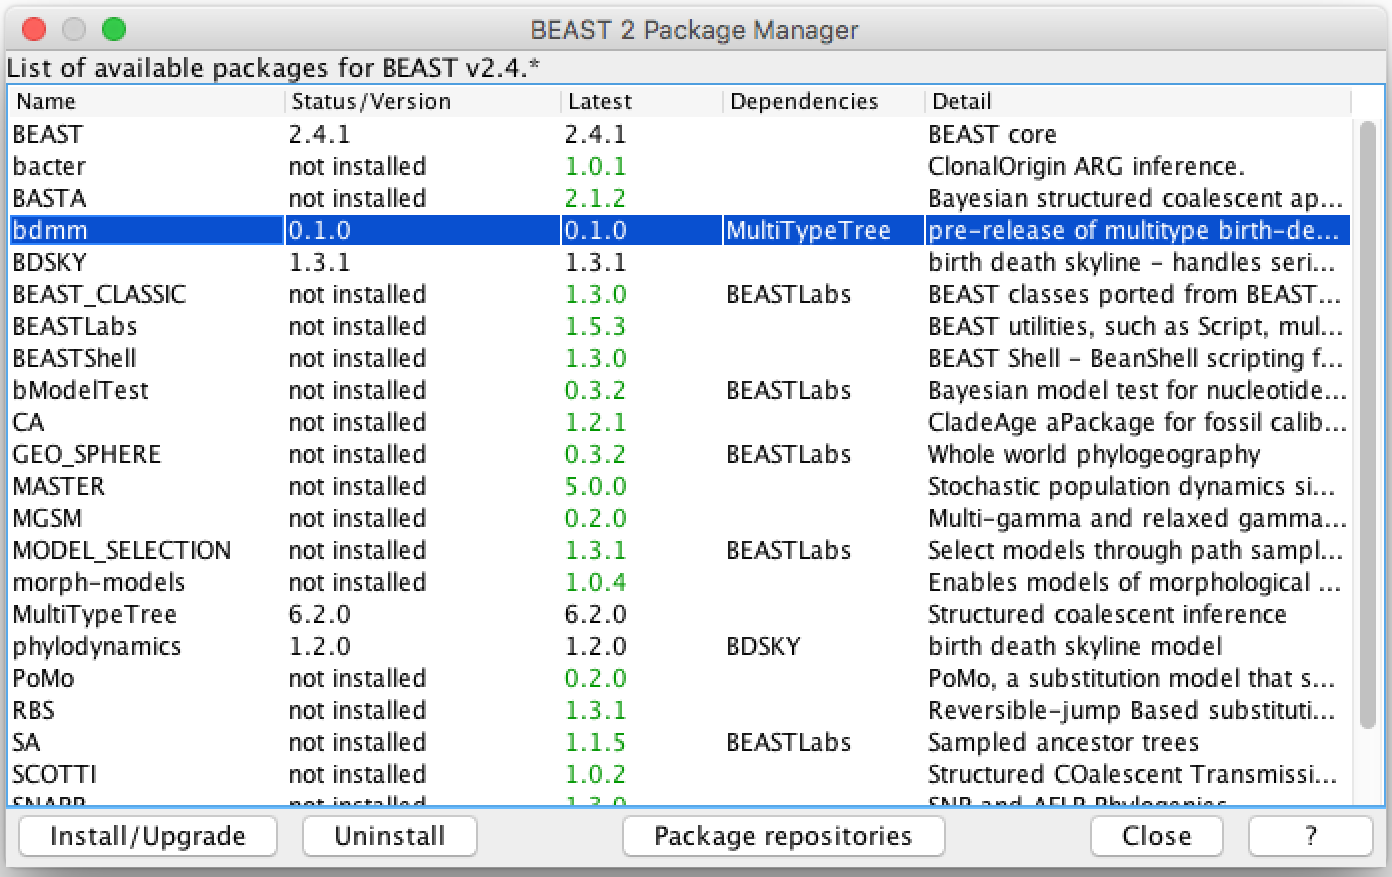
\includegraphics[width=0.750000\textwidth]{figures/1-install-bdmm.png}
    \caption{Install bdmm.}
    \label{fig:}
\end{figure}

(Note the actual version of bdmm may differ from the version shown in
the figure. This is normal.)

Finally, \textbf{restart BEAUti.} This is very important. Strange
behaviour may result if you do not restart the program.

\section{Setting up the analysis using
BEAUti}\label{setting-up-the-analysis-using-beauti}

\subsection{Loading the Template}\label{loading-the-template}

A BEAUTI template defines the basic structure and contents of your XML
file. Because by default BEAUTI will construct an XML file with standard
BEAST trees, rather than MultiTypeTrees, we cannot use the default
template (Standard.xml). Hence, from the \emph{File} menu, select
\emph{Template} and then choose \emph{MultiTypeBirthDeath}.

\begin{figure}
    \centering
    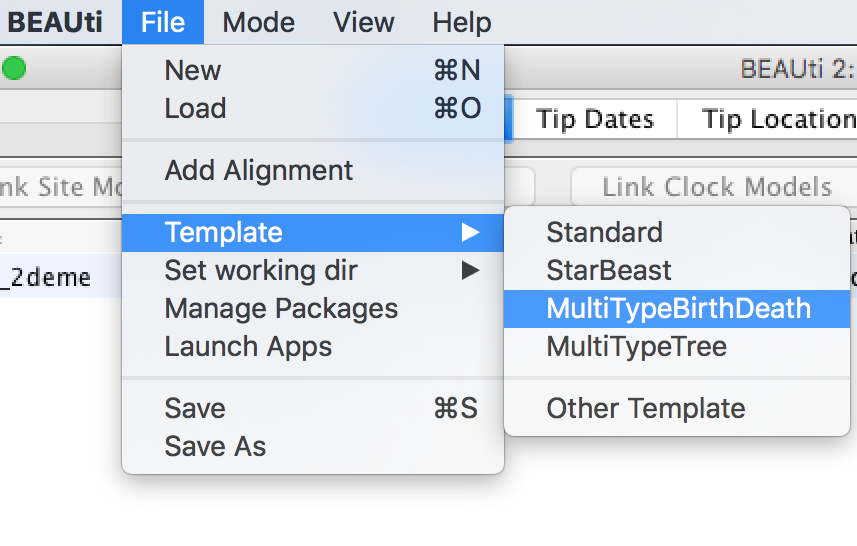
\includegraphics[width=0.500000\textwidth]{figures/2-choose-bdmm-template.png}
    \caption{Load the MultiTypeBirthDeath template.}
    \label{fig:}
\end{figure}

\subsection{Loading the data}\label{loading-the-data}

Once the template is loaded, we can load in our example sequence data.
In our case, this data is stored in a FASTA file, the first few lines of
which look like this:

\begin{lstlisting}
> EU856841_HongKong_2005.34246575
-----------GGGATAATTCTATTAACCATGAAGACTATCATTGCTTTGAGCTACATTT
> EU856989_HongKong_2002.58356164
--CAAAAGCAGGGGATAATTCTATTAACCATGAAGACTATCATTGCTTTGAGCTACATTT...
> CY039495_HongKong_2004.5890411
------------------TTCTATTAACCATGAAGACTATCATTGCTTTGAGCTACATTC...
> EU856853_HongKong_2001.17808219
---------------------TATTAACCATGAAGACTATCATTGCTTTGAGCTACATTC...
> CY010084_NewZealand_2005.62739726
---------------------TATTAACCATGAAGACTATCATTGCTTTGAGCTACATTC...
> CY007387_NewZealand_2004.63287671
---------------------TATTAACCATGAAGACTATCATTGCTTTGAGCTACATTC...
> CY012432_NewZealand_2000.81643836
---------------------------CCATGAAGACTATCATTGCTTTGAGCTACATTT...
\end{lstlisting}

The lines beginning with ``\textgreater{}'' are labels for the sequences
immediately following. In general, these labels have no special format,
but in this file each label is an underscore-delimited triple. The first
element of each triple is the GenBank accession number of the sequence,
the second is the geographical region from which it was sampled, and the
third is the time at which it was sampled measured in calendar years or
fractions thereof. (The ellipses are not in the file, but are used here
to indicate that sequence has been truncated.)

In this tutorial we will be using the influenza sequence data which is
distributed with MultiTypeTree. To make this easy to find, open the
\emph{File} menu and select \emph{Set working dir}. Then, from the
submenu that appears, select \emph{MultiTypeTree}.

\begin{figure}
    \centering
    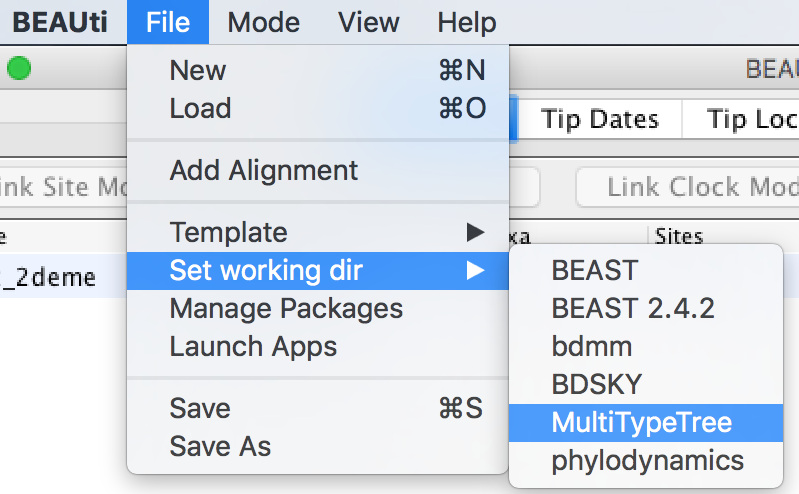
\includegraphics[width=0.500000\textwidth]{figures/3-set-working-dir.png}
    \caption{Set the working directory to MultiTypeTree.}
    \label{fig:}
\end{figure}

(This step is not required when loading your own data.)

To load the file, open the \emph{File} menu and select \emph{Add
alignment}. This will open a file selection dialog box. The example
influenza sequence data file is named \lstinline!h3n2_2deme.fna!.
Assuming you have followed the previous step to set the working
directory, this can be found in the \lstinline!examples/! directory
shown when the file selection dialog box loads.

Once this file is loaded, your BEAUti screen should look something like
the following:

\begin{figure}
    \centering
    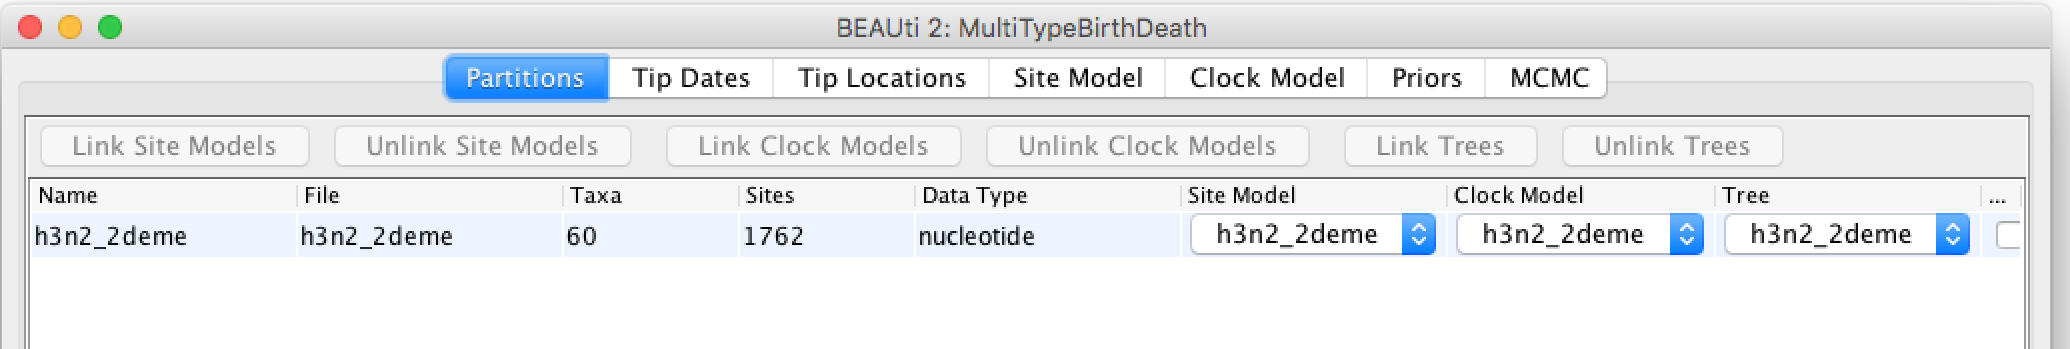
\includegraphics[max width=\textwidth, max height=0.9\textheight]{figures/4-alignment-loaded.png}
    \caption{The alignment loaded into BEAUti.}
    \label{fig:}
\end{figure}

\subsection{Setting up dates}\label{setting-up-dates}

Once the data is loaded, the next step is to specify the times at which
the sequences were sampled:

\begin{enumerate}
\def\labelenumi{\arabic{enumi}.}

\item
  Select the ``Tip Dates'' panel.
\item
  Check the ``Use tip dates'' checkbox.
\item
  Click the ``Guess'' button at the top-right of the panel. This opens a
  dialog that allows sample times to be loaded from a file or inferred
  (guessed) from the sequence labels.
\item
  Because the times are included as the last element of the
  underscore-delimited sequence names, choose the ``use everything''
  radio button and select ``after last'' from the drop-down menu. (Note
  that the underscore character is already chosen as the delimiter.)
\end{enumerate}

\begin{figure}
    \centering
    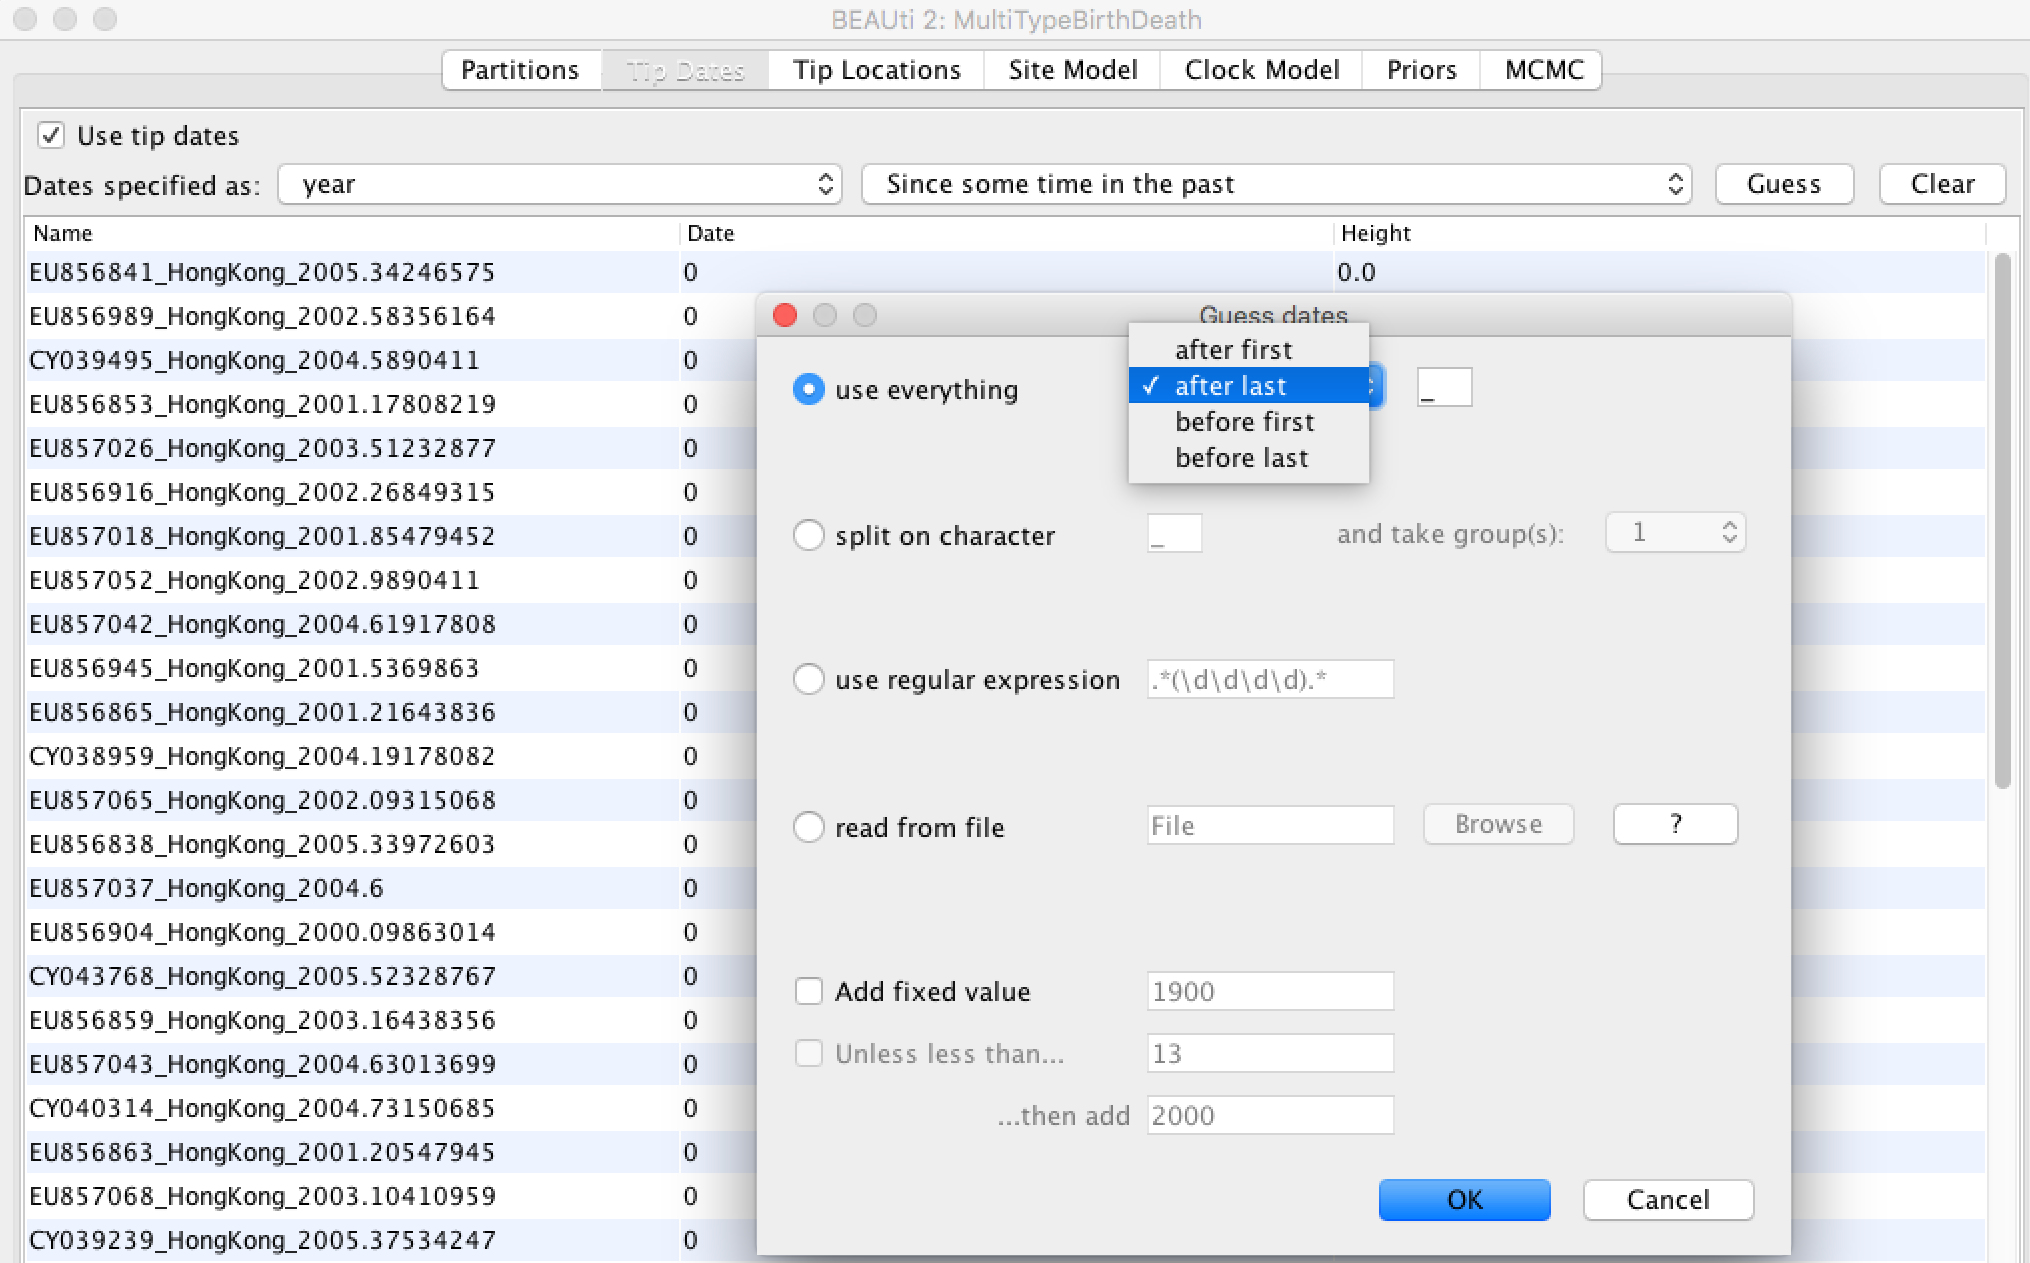
\includegraphics[max width=\textwidth, max height=0.9\textheight]{figures/5-tip-dates.png}
    \caption{Guessing the tip-dates.}
    \label{fig:}
\end{figure}

After clicking ``OK'' you should find that the tip date table is
populated with times that match those in the sequence headers, and that
the last column of the table contains ``heights'' (times before most
recent sample) calculated from the times:

\begin{figure}
    \centering
    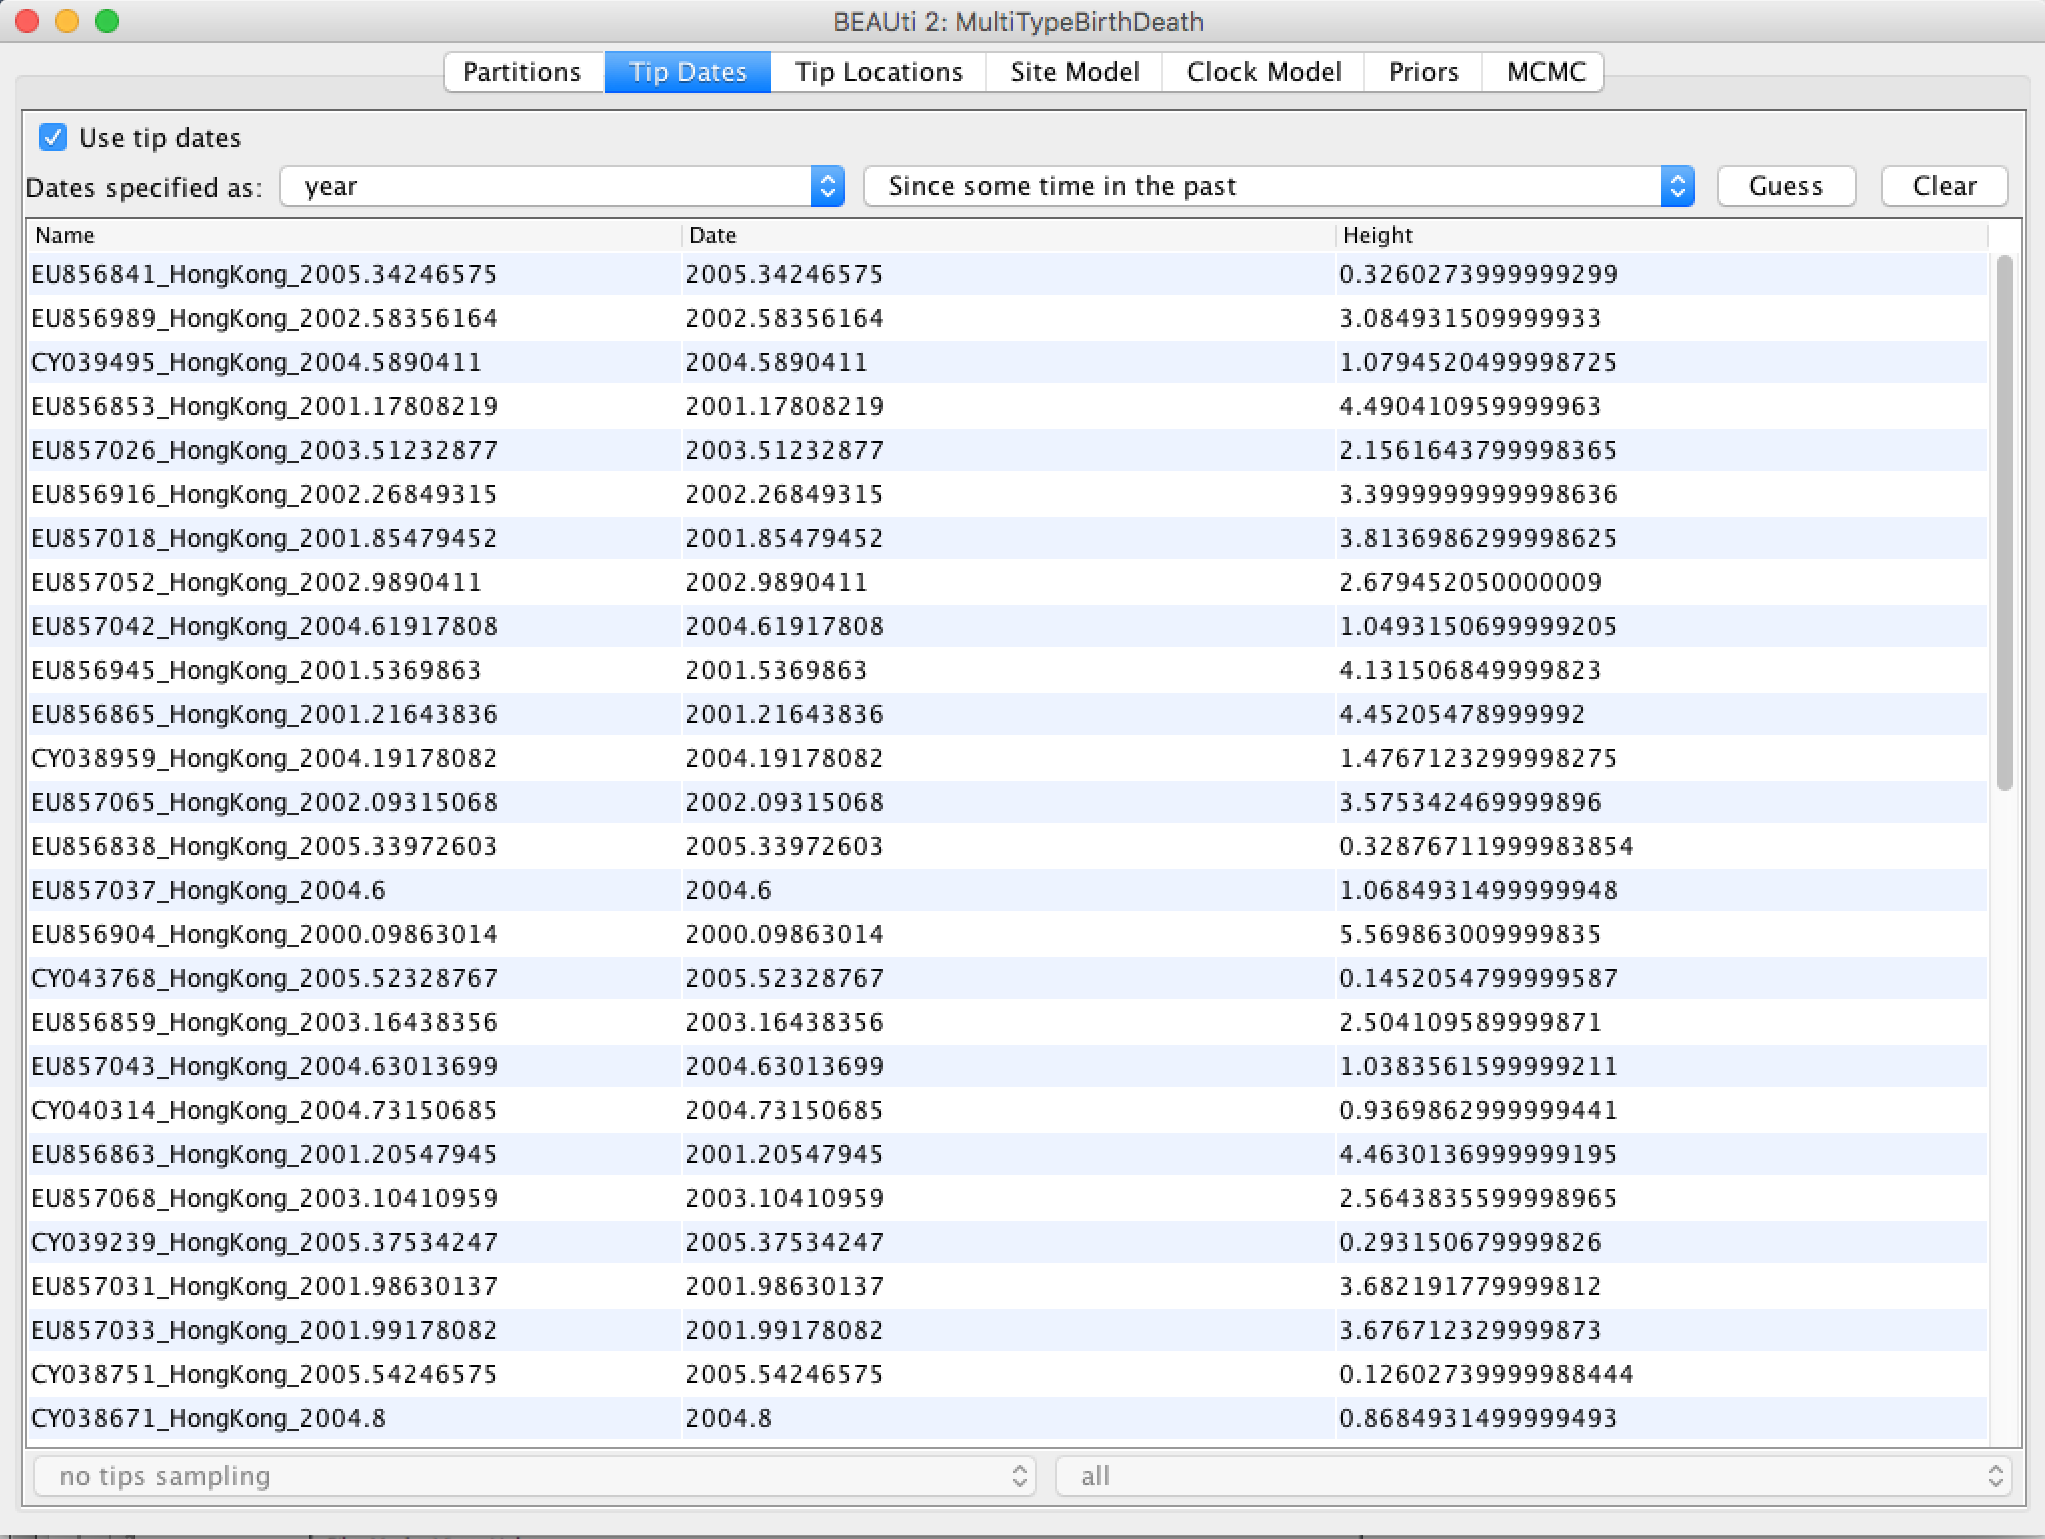
\includegraphics[max width=\textwidth, max height=0.9\textheight]{figures/5b-tip-dates-set.png}
    \caption{Sampling dates in BEAUti.}
    \label{fig:}
\end{figure}

\subsection{Setting up locations}\label{setting-up-locations}

Now that we've specified the sampling times, we move on to specifying
the sampling locations. To do this, we follow a very similar set of
steps to those we used to set the sample times:

\begin{enumerate}
\def\labelenumi{\arabic{enumi}.}

\item
  Select the ``Tip Locations'' panel. You'll find that the locations are
  already populated with default values.
\item
  Click the ``Guess'' button at the top-right of the panel. This opens
  the same dialog that we saw in the previous section.
\item
  Because the locations are included as the second element of the
  underscore-delimited sequence names, choose the ``split on character''
  radio button and select group 2 from the drop-down menu. (Note again
  that the underscore character is already chosen as the delimiter.)
\end{enumerate}

\begin{figure}
    \centering
    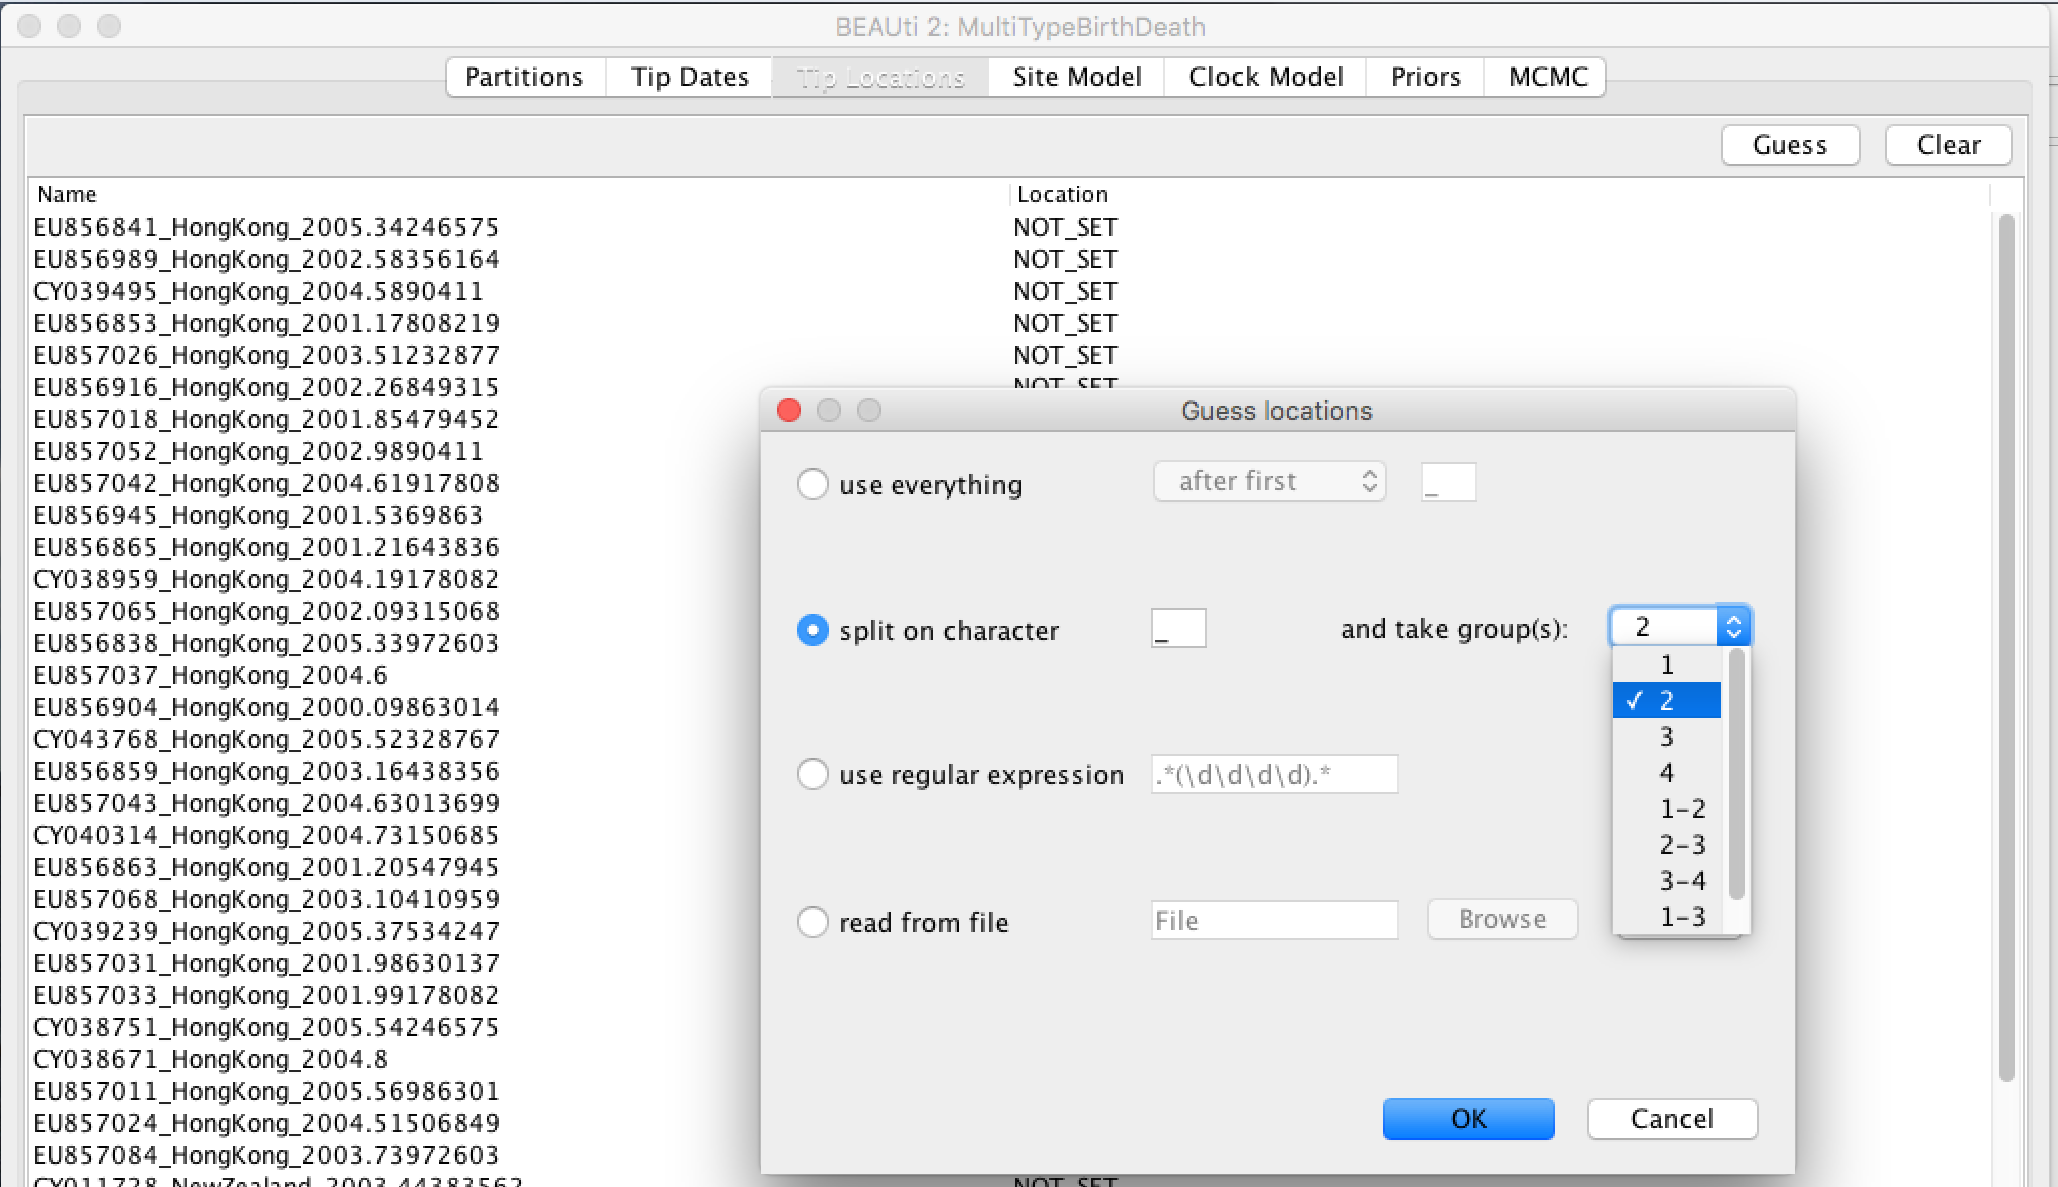
\includegraphics[max width=\textwidth, max height=0.9\textheight]{figures/6-tip-types.png}
    \caption{Guessing the locations.}
    \label{fig:}
\end{figure}

After clicking ``OK'' you should find that the tip location table is
populated with locations that match those in the sequence headers, as
follows:

\begin{figure}
    \centering
    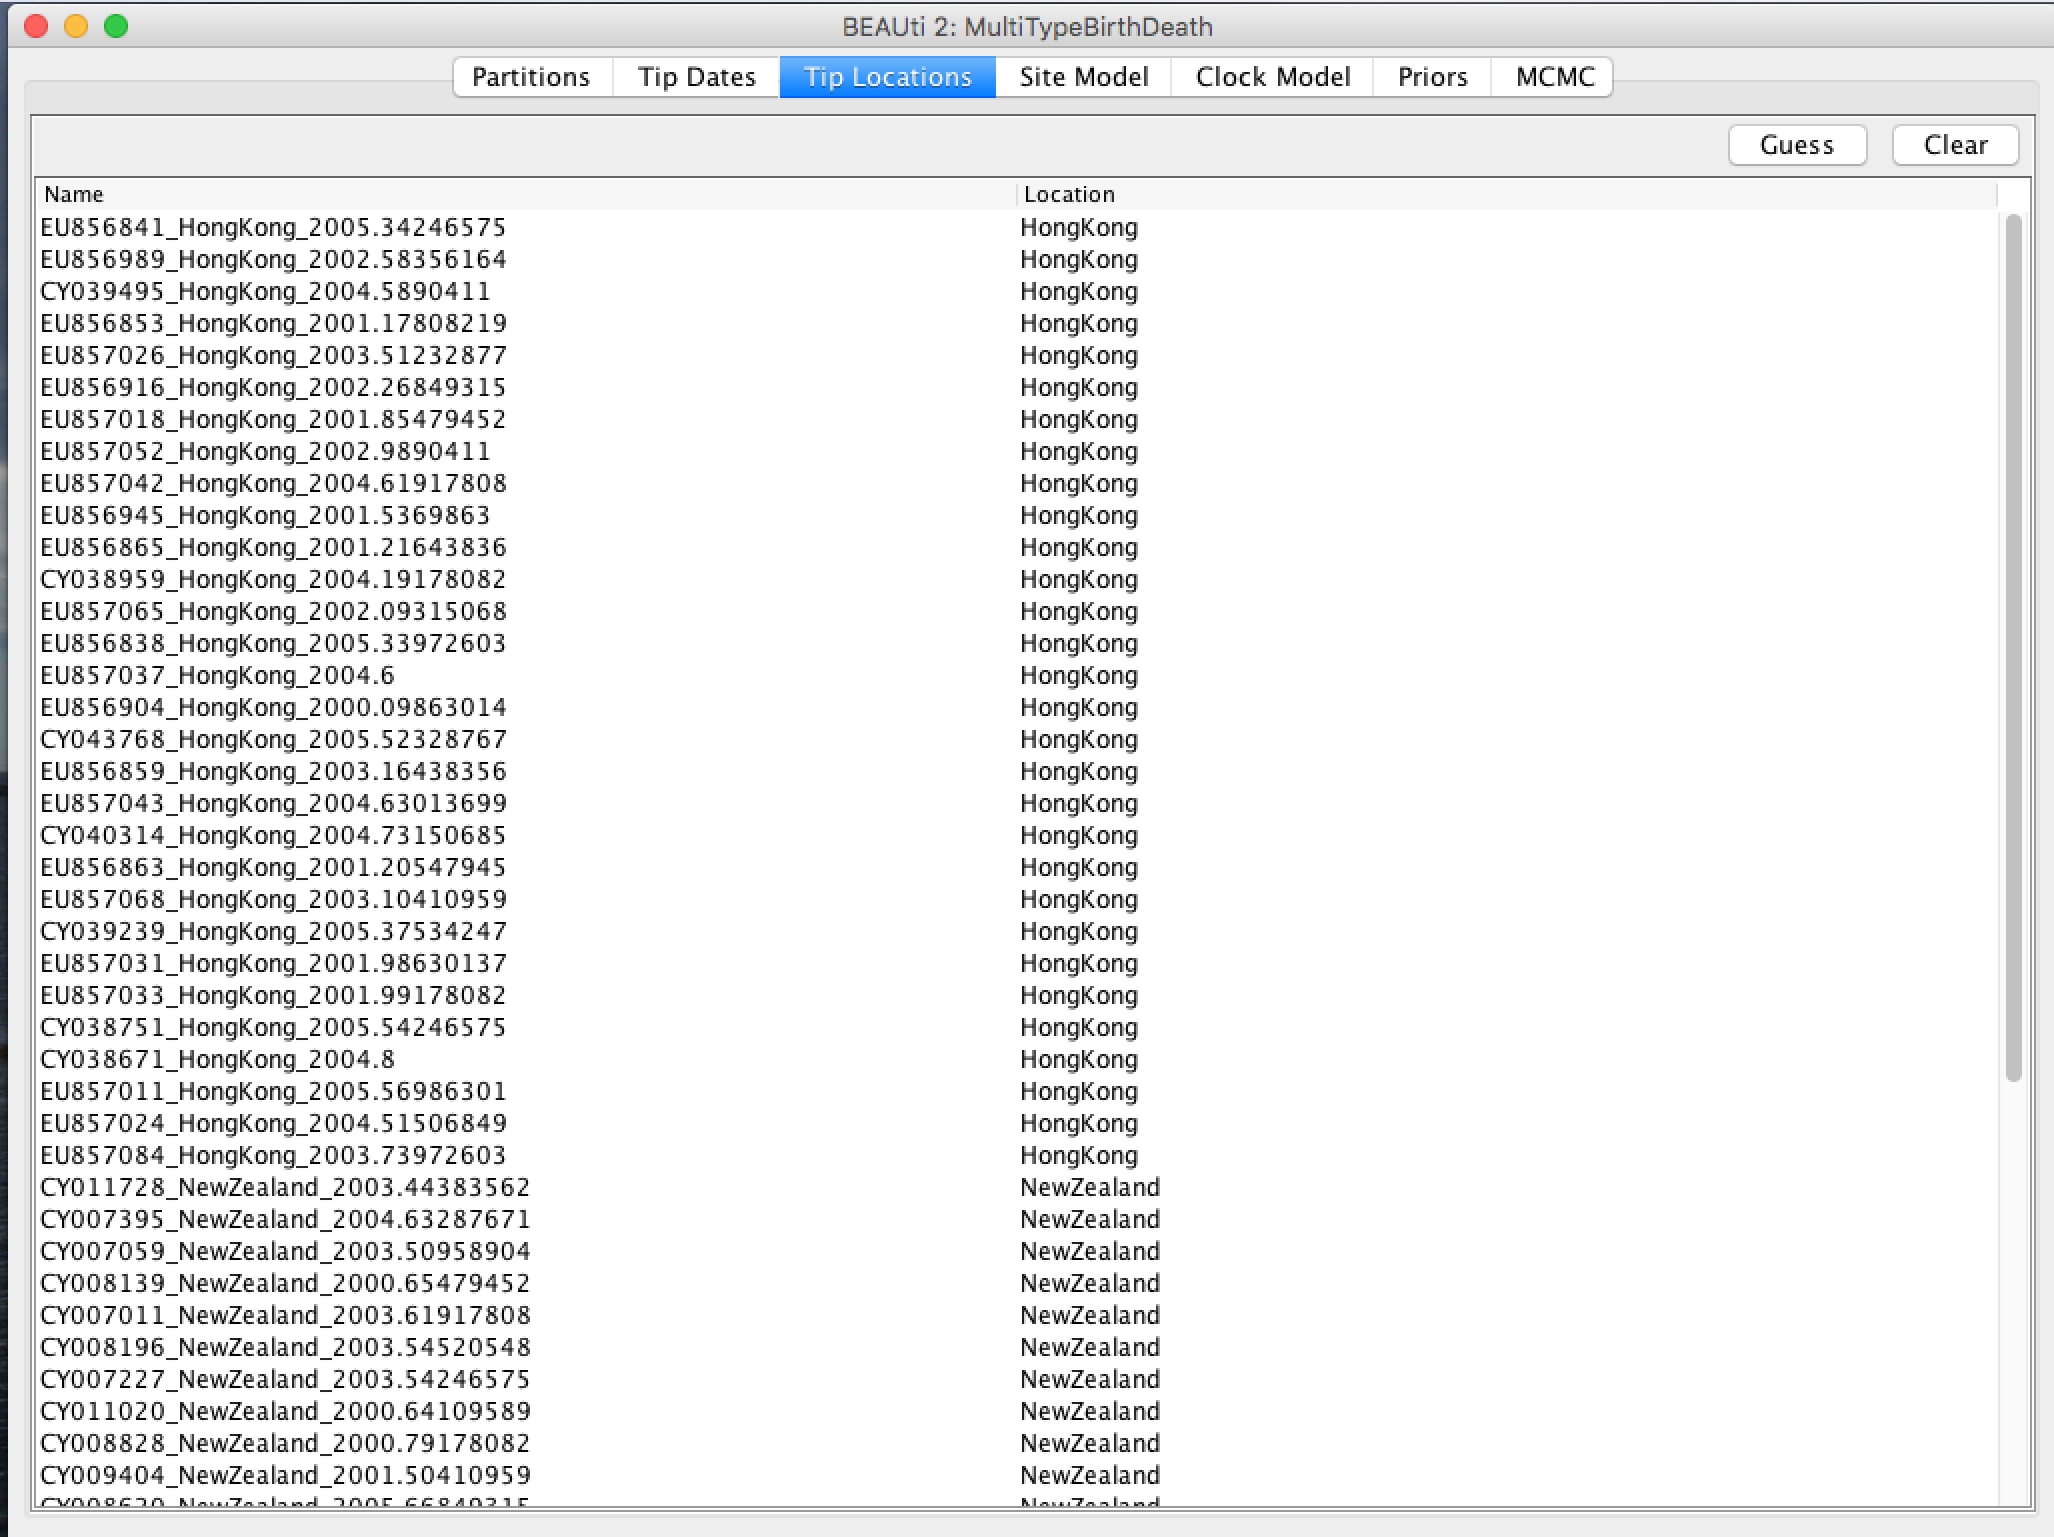
\includegraphics[max width=\textwidth, max height=0.9\textheight]{figures/6b-tip-types-set.png}
    \caption{The locations in BEAUti.}
    \label{fig:}
\end{figure}

\subsection{Substitution model}\label{substitution-model}

For this analysis, we will use the HKY substitution model with 4 gamma
categories and estimated base frequencies. To configure this in BEAUti,
switch to the ``Site Model'' panel, change the number of gamma
categories and select HKY from the drop-down menu (the default option is
JC69). We also want the shape and proportionInvariant parameters to be
nonzero and estimated to account for heterogeneity between sites in our
alignment.

The BEAUti panel should now look like the following:

\begin{figure}
    \centering
    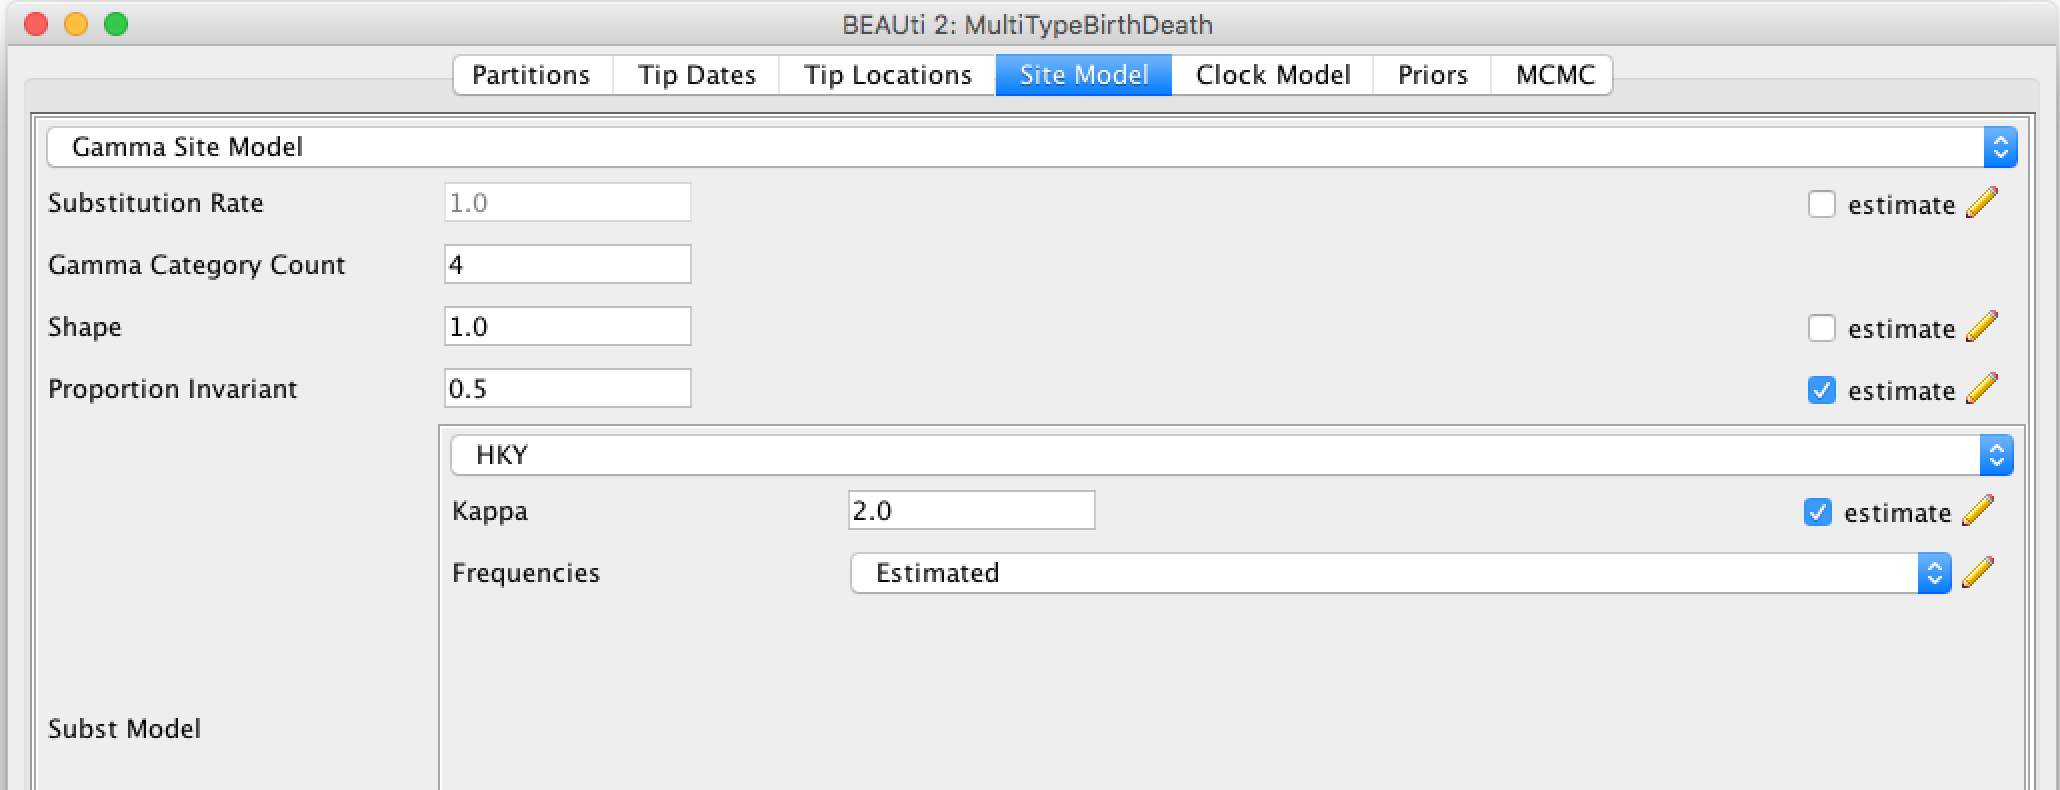
\includegraphics[max width=\textwidth, max height=0.9\textheight]{figures/7-sitemodel.png}
    \caption{Setup of the site model.}
    \label{fig:}
\end{figure}

Note that the ``Substitution rate'' defined on this panel should be left
non-estimated - we use the ``Clock rate'' defined in the ``Clock Model''
panel to determine the average per unit time rate of sequence evolution.
Used this way, the ``substitution rate'' is therefore not actually a
rate (it's actually dimensionless) but is instead a rate multiplier that
in our case we fix at 1.

\subsection{Defining Clock model}\label{defining-clock-model}

For this analysis we assume a strict clock. Since our alignment contains
sequences sampled at different times and those times are measured in
years, we must use a real clock rate expressed in units of expected
substitutions per site per year. Usually the precise value is unknown
and so the default behaviour of BEAUti is to assume this rate is to be
estimated. We set the clock rate to 0.005, which we know is much closer
to the truth than the default 1, to speed up mixing. The Clock Model
panel should now look like this:

\begin{figure}
    \centering
    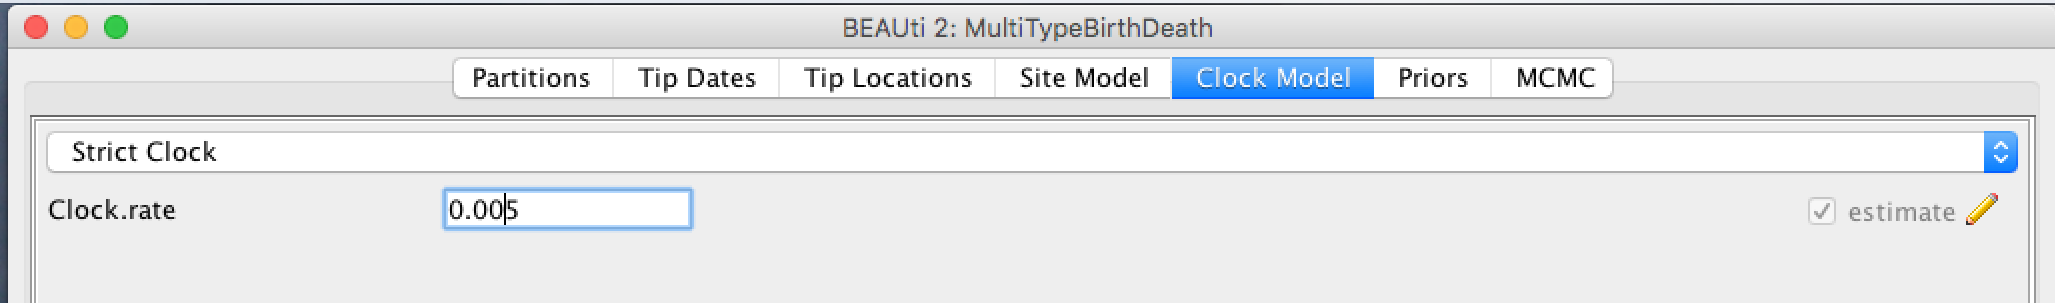
\includegraphics[max width=\textwidth, max height=0.9\textheight]{figures/8-strict-clock.png}
    \caption{Fix the clock rate to speed up mixing.}
    \label{fig:}
\end{figure}

\subsection{Adjusting Priors}\label{adjusting-priors}

Because bdmm is a model-based prior on the (multi-type) tree
distribution, setting up the ``Priors'' panel is a particularly
important part of setting up this analysis.

It is important to change the time at which sampling started, counting
from the time of the last sample. In our case, the time between the
first and last sample is 5.57 (rounded UP). Note, that the sampling
proportion has 4 entries, let's call them {[}s11,s12,s21,s22{]}. The
values s11 and s12 belong to type 1 (HongKong) and s21, s22 belong to
type 2 (New Zealand). The values s11 and s21 belong to the first
interval, which is the time before the first sample, which is why
s11=s21=0.

\begin{figure}
    \centering
    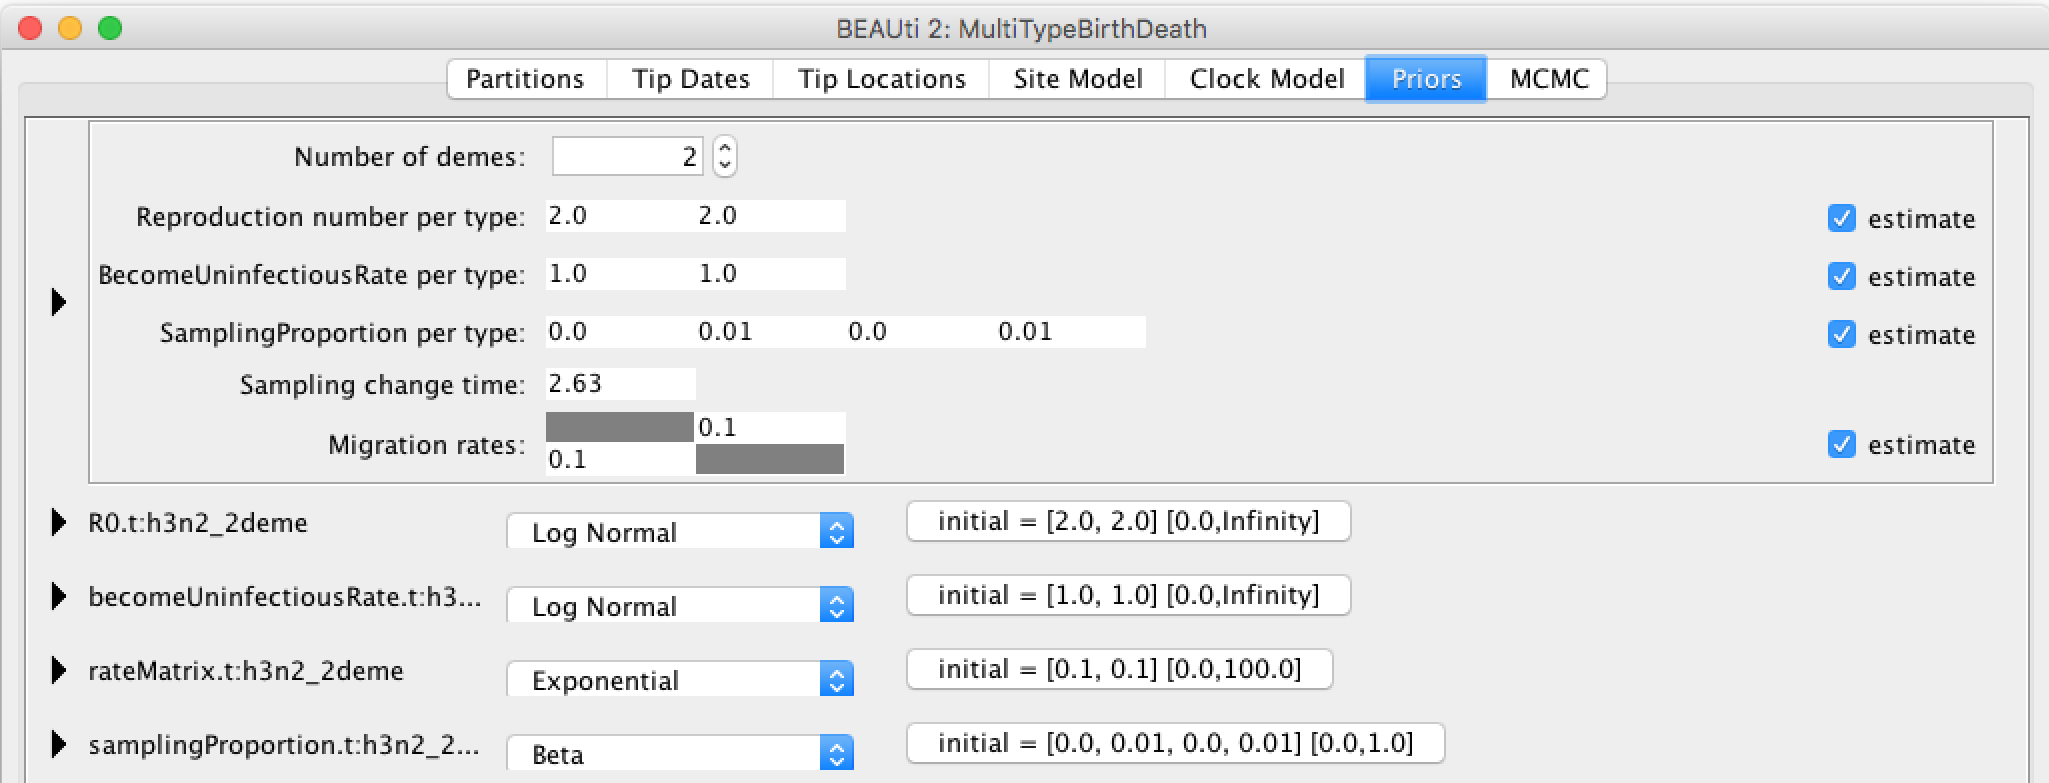
\includegraphics[max width=\textwidth, max height=0.9\textheight]{figures/9-priors.png}
    \caption{Set the change time for the sampling proportion so it is zero before the time of the first sample.}
    \label{fig:}
\end{figure}

When you expand the tree prior element, you can change the condition on
survival setting. We'll leave the box checked.

\begin{figure}
    \centering
    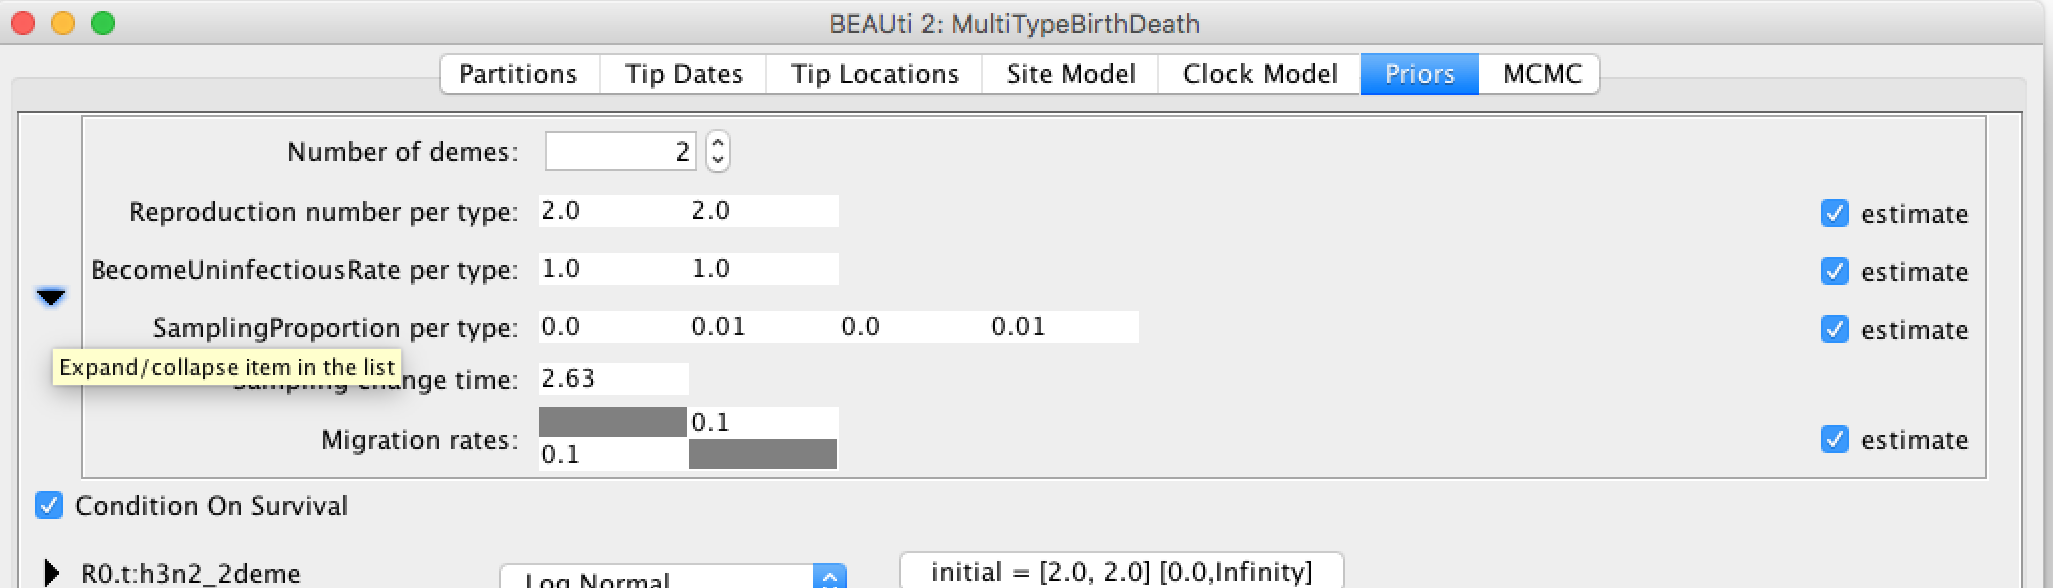
\includegraphics[max width=\textwidth, max height=0.9\textheight]{figures/9b-condition.png}
    \caption{Condition on survival.}
    \label{fig:}
\end{figure}

Ensure the value shown in the ``State Number'' spinner is equal to the
number of types present in your model. In this case, the default value
of 2 is correct, but in general you should check your data and change
this value accordingly.

Click the arrows on the left-hand side of each parameter to alter the
details of these priors. For example, we will set the rateMatrix prior
distribution to Exp(1):

\begin{figure}
    \centering
    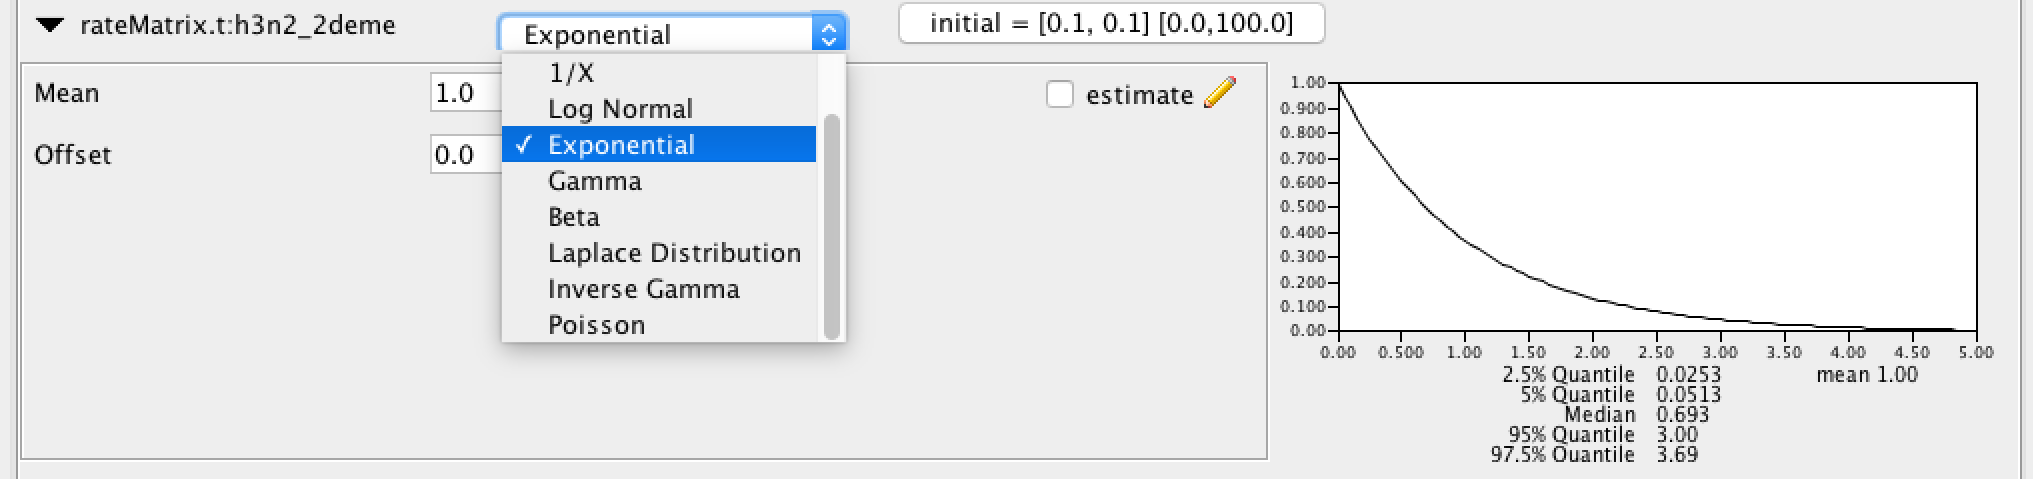
\includegraphics[max width=\textwidth, max height=0.9\textheight]{figures/9d-prior-rateMatrix.png}
    \caption{Set the prior for the rate matrix.}
    \label{fig:}
\end{figure}

We will use the default set-up for the MCMC and save our file as usual.

\section{Running the analysis using
BEAST}\label{running-the-analysis-using-beast}

To run the analysis, simply start BEAST 2 in the manner appropriate for
your platform, then select the file you generated in the last section as
the input file. (Refer to the documentation provided at
\href{http://www.beast2.org/}{www.beast2.org} for detailed
instructions.)

\section{Analyzing the results}\label{analyzing-the-results}

The results of the analysis primarily consist of two parts:

\begin{enumerate}
\def\labelenumi{\arabic{enumi}.}

\item
  The parameter log, which is written to the file
  \lstinline!h3n2-bdmm-v2-samplingPrior.log!.
\item
  The tree log, which is written to
  \lstinline!h3n2-bdmm-v2-samplingPrior.h3n2_2deme.trees!.
\end{enumerate}

In addition, the file
\lstinline!h3n2-bdmm-v2-samplingPrior.h3n2_2deme.map.trees! contains the
running estimate of the MAP tree as a function of MCMC step number,
while the file
\lstinline!h3n2-bdmm-v2-samplingPrior.h3n2_2deme.typedNode.trees! is the
TreeAnnotator-compatible file we'll use to assemble a summary tree.

\subsection{Parameter log file
analysis}\label{parameter-log-file-analysis}

We can use the program
\href{http://tree.bio.ed.ac.uk/software/tracer/}{Tracer} to view the
parameter log file. To do this, start Tracer and then press the ``+''
button in the top-left hand corner of the window (under ``Trace
files''). Select the log file for this analysis
(\lstinline!h3n2_2deme.log!) from the file selection dialog box. The
``Traces'' table will then be populated with parameters and summary
statistics corresponding to our multitype birth-death analysis.

Important traces are: * \lstinline!R0.t:h3n2_2deme1! and
\lstinline!R0.t:h3n2_2deme2!: These give the effective reproduction
numbers for deme 1 (Hongkong) and 2 (New Zealand), respectively.

\begin{itemize}
\item
  \lstinline!rateMatrix.t:h3n2_2deme1!
  \lstinline!rateMatrix.t:h3n2_2deme2!: These give the (per lineage per
  year) migration rates from deme 1 to 2 and vice versa.
\item
  \lstinline!Tree.t:h3n2_2deme.count_HongKong_to_NewZealand!: these give
  the actual number of ancestral migrations from HongKong to New
  Zealand.
\end{itemize}

The panels tabs at the top-right of the window can be used to display
one or more selected traces in various ways. For example, selecting the
two R0 traces and choosing the ``Marginal prob distribution'' panel
results in the following useful comparison between the sampled
population size marginal posterior distributions:

\begin{figure}
    \centering
    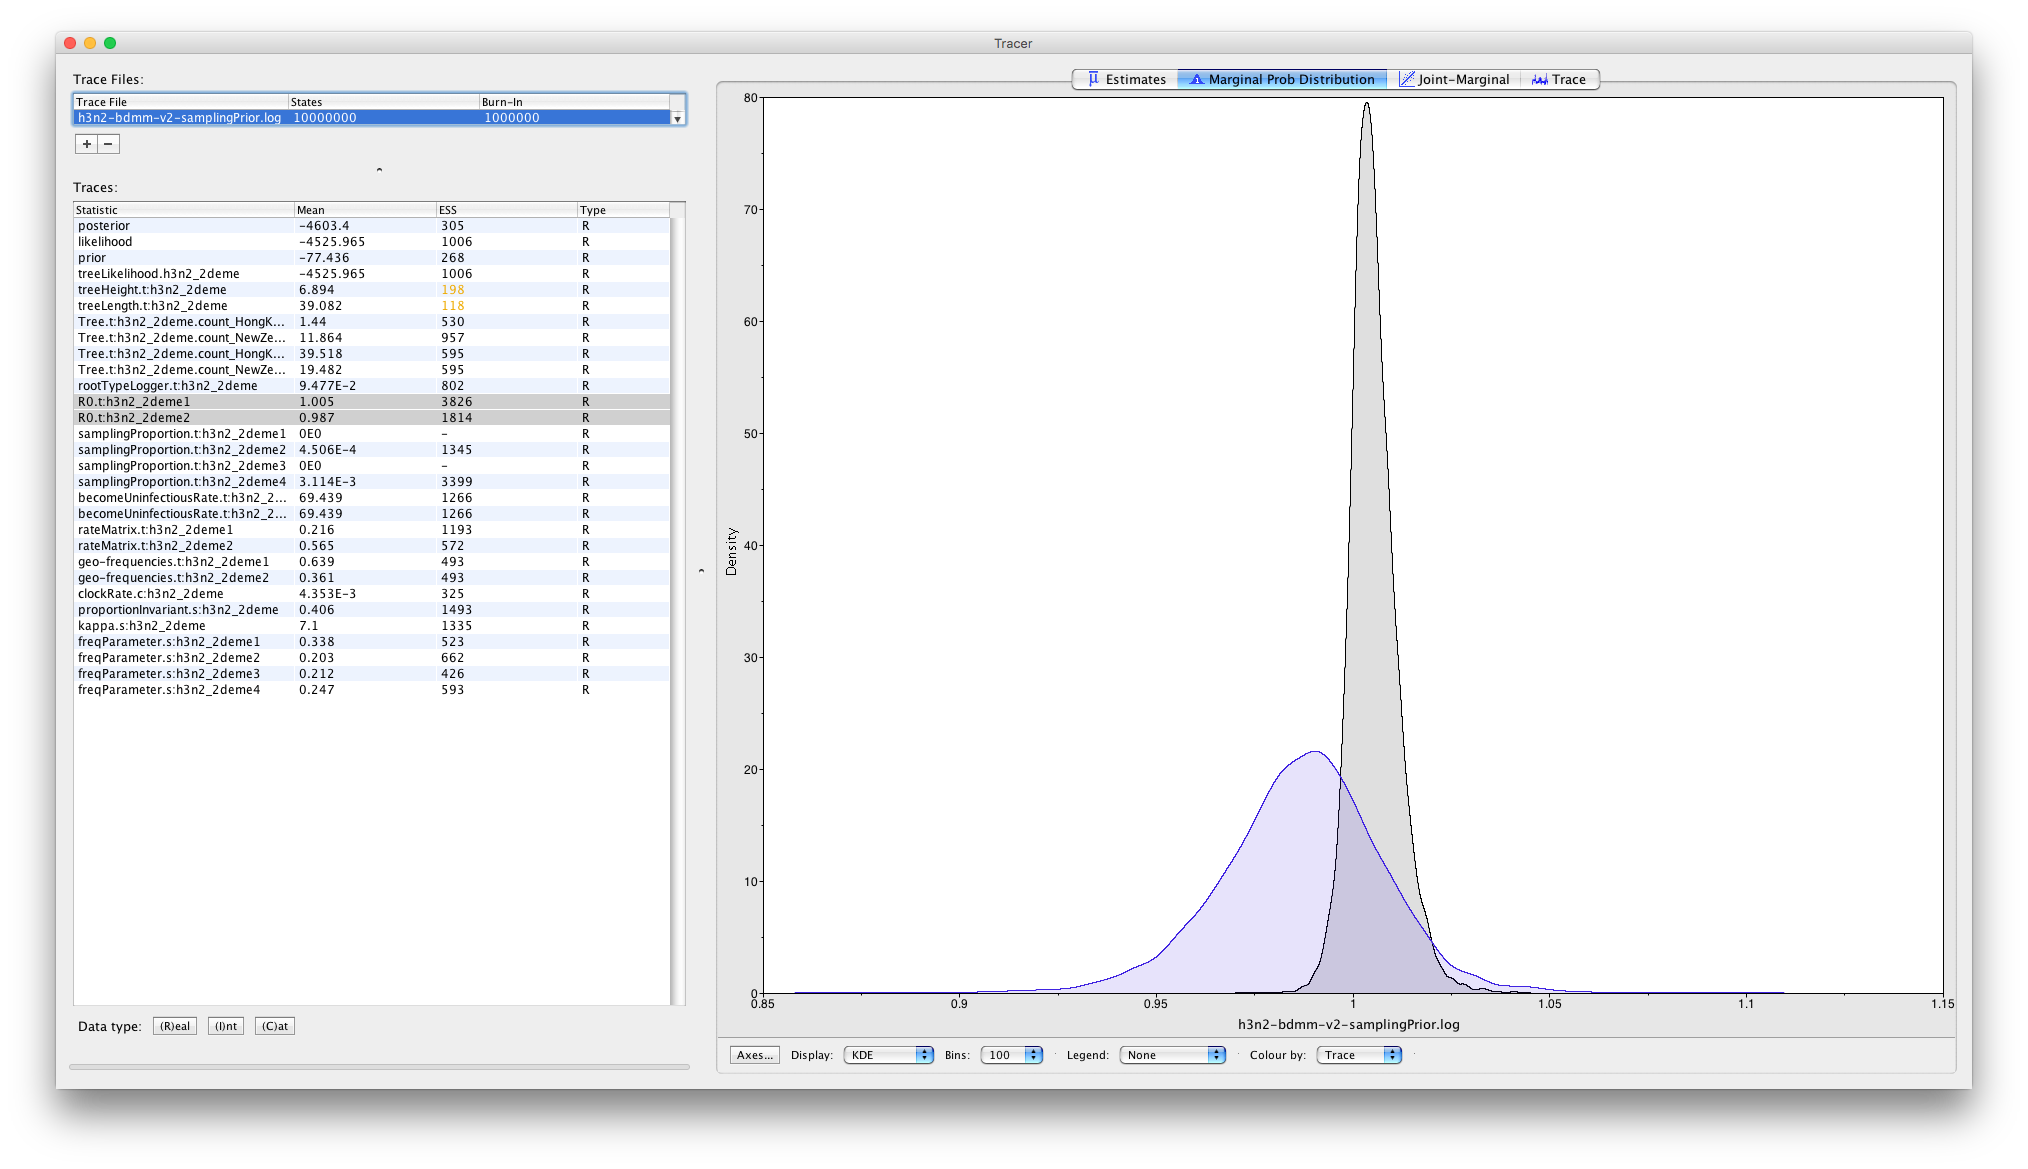
\includegraphics[max width=\textwidth, max height=0.9\textheight]{figures/tracer-R0.png}
    \caption{Estimated `$ R_0 $` marginal posteriors.}
    \label{fig:}
\end{figure}

Note that some of the ESS values are still less than 200 - the arbitrary
threshold for acceptability. If this analysis were part of a serious
study you would want to run the chain for another few million iterations
to improve these. (In BEAST 2, analyses can be resumed - the samples
you've already acquired will not be wasted.) For the purposes of this
tutorial, however, these values are acceptable.

\subsection{Tree log visualization}\label{tree-log-visualization}

The popular phylogenetic tree visualizer
\href{http://tree.bio.ed.ac.uk/software/figtree/}{FigTree} can be used
to visualize the sampled trees. Be warned, however, that FigTree
currently takes an extremely long time to load even relatively small (a
few megabyte) MultiTypeTree logs.

For this reasons we suggest using
\href{http://tgvaughan.github.io/icytree}{IcyTree} to view tree log
files and maybe switching to FigTree to visualize summary trees as
discussed in the next section. (Also, IcyTree can be used to export
individual trees from a large log file for subsequent viewing using
FigTree.) IcyTree is a tree viewer that runs in a web browser. It runs
best under recent versions of \href{http://www.google.com/chrome}{Google
Chrome} and \href{https://www.mozilla.org/en-US/firefox/}{Mozilla
Firefox} (in that order).

To view MultiTypeTree log files using IcyTree, simply navigate to the
IcyTree web page, select ``Load from file'' from the ``File'' menu, then
select one of the tree log files using the file selection dialog. Once
the file is loaded you will see the first tree it contains. In order to
select a different tree, move the mouse pointer over the box in the
lower-left corner of the window. This box will expand to a small dialog
containing buttons allowing you to navigate between trees. The
`\textless{}' and `\textgreater{}' buttons move in steps of 1 tree,
while `\textless{}\textless{}' and `\textgreater{}\textgreater{}' move
10\% of the tree file per click. You can also directly enter the index
of a tree. (Note that there are keyboard shortcuts for almost all
commands in IcyTree and that these can be found by selecting ``Keyboard
shortcuts'' from the ``Help'' menu.)

Initially the trees edges will be uncoloured. To colour the edges
according to the edge type, open the ``Style'' menu, navigate to the
``Colour edges by'' submenu and select ``type''. A legend and axis can
be added by choosing ``Display legend'' and ``Axis \textgreater{} Age''
from the same menu.

The following shows the final tree of
\lstinline!h3n2-bdmm-v2-samplingPrior.h3n2_2deme.map.trees! in IcyTree,
which represents our sampled estimate of the MAP multi-type tree:

\begin{figure}
    \centering
    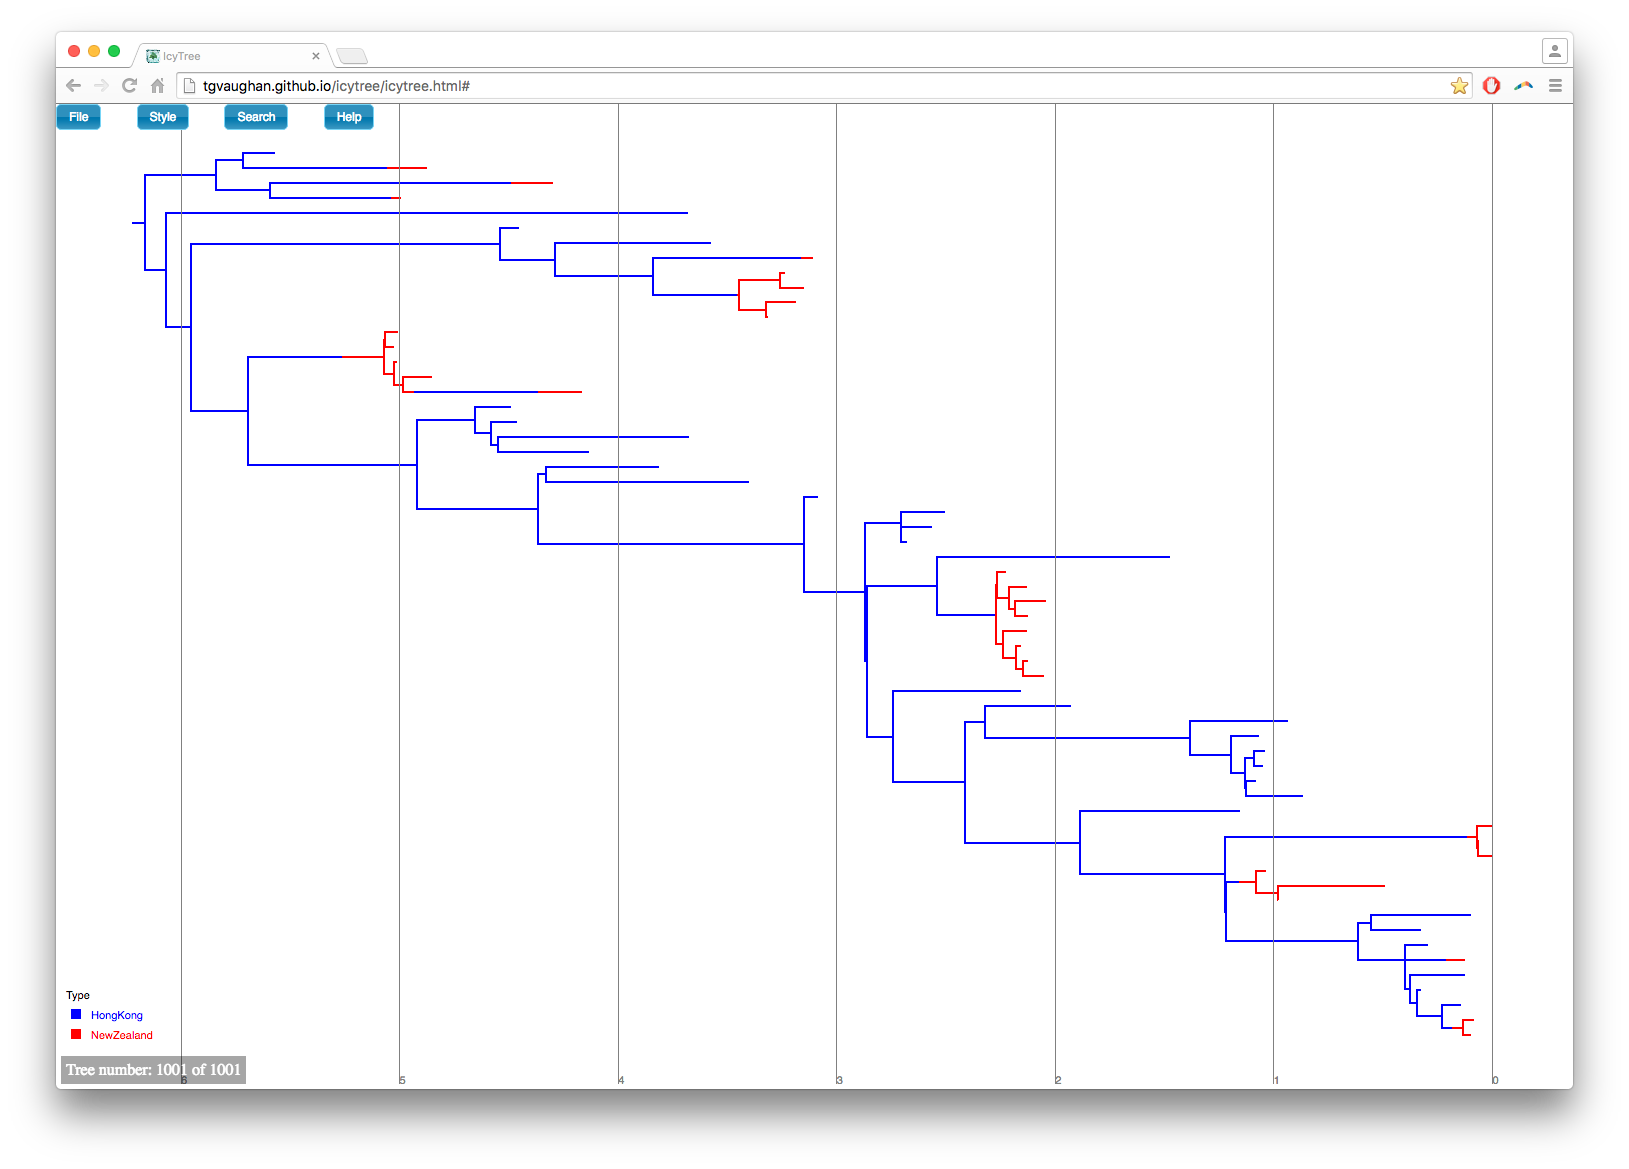
\includegraphics[max width=\textwidth, max height=0.9\textheight]{figures/icyTreeMAP.png}
    \caption{The MAP multi-type tree in IcyTree.}
    \label{fig:}
\end{figure}

While IcyTree is useful for rapidly visualizing the results of an
analysis, it is not nearly as feature-rich as FigTree and not as capable
for producing publication-quality graphics. Happily, however, IcyTree
can extract single trees from larger log files. Simply navigate to the
desired tree, open the ``File'' menu, choose the ``Export tree as''
submenu and select ``NEXUS file''. (It is important to select ``NEXUS''
instead of ``Newick'' as the Newick format does not support the
annotations that MultiTypeTree uses to mark the edge types.)

\subsection{Producing a summary tree using
TreeAnnotator}\label{producing-a-summary-tree-using-treeannotator}

While it is tempting to view the MAP tree shown above as the primary
result of the phylogenetic side of our analysis it is very important to
remember that this is only a point estimate and says nothing about the
uncertainty present in the result. This is an important drawback, as we
have done a full Bayesian analysis and have access to a large number of
samples from the full posterior in the tree log files. The MAP tree
discards almost all of this information.

We can make better use of our raw analysis results by using the
TreeAnnotator program which is distributed with BEAST to analyze the
\lstinline!typedNode! trees which were produced by our MCMC run. To do
this, simply load TreeAnnotator and select the \lstinline!typedNode!
tree file as the input file and
\lstinline!h3n2-bdmm-v2-samplingPrior.h3n2_2deme.summary.trees! as the
output file. Select ``Mean heights'' from the ``Node heights'' menu and
set the burn-in percentage to 10:

\begin{figure}
    \centering
    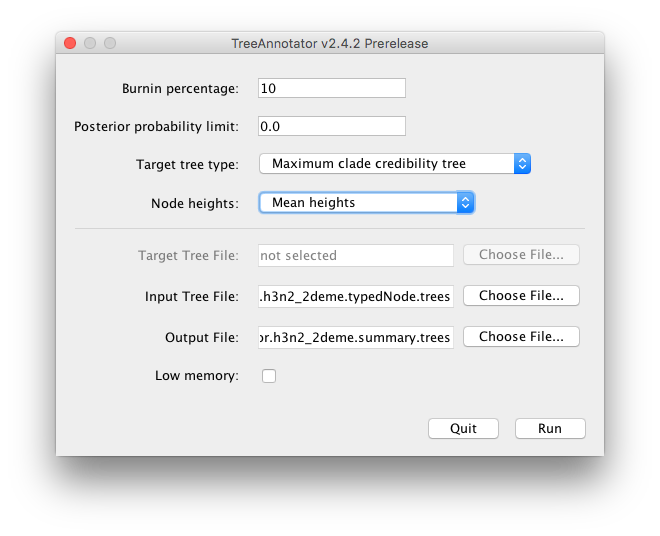
\includegraphics[width=0.500000\textwidth]{figures/treeannotator.png}
    \caption{Use TreeAnnotator to produce a summary tree.}
    \label{fig:}
\end{figure}

Pressing the ``Run'' button will now produce an annotated summary tree.

To visualize this tree, open IcyTree once more (maybe open it in a new
browser tab), choose File-\textgreater{}Open, then select the file
\lstinline!h3n2_2deme.h3n2_2deme.summary.tree! using the file selection
dialog. Follow the instructions provided for the MAP tree above to
colour the tree by the ``type'' attribute and add the legend and time
axis. In addition, open the Style menu and from the ``Node height error
bars'' sub-menu select ``height\_95\%\_HPD" to add error bars to the
internal node heights. Also, open the Style menu and from the ``Edge
opacity'' sub-menu select ``type.prob''. This will cause the edges to
become increasingly transparent as the posterior probability for the
displayed colour decreases.

Once these style preferences have been set, you should see something
similar to the following:

\begin{figure}
    \centering
    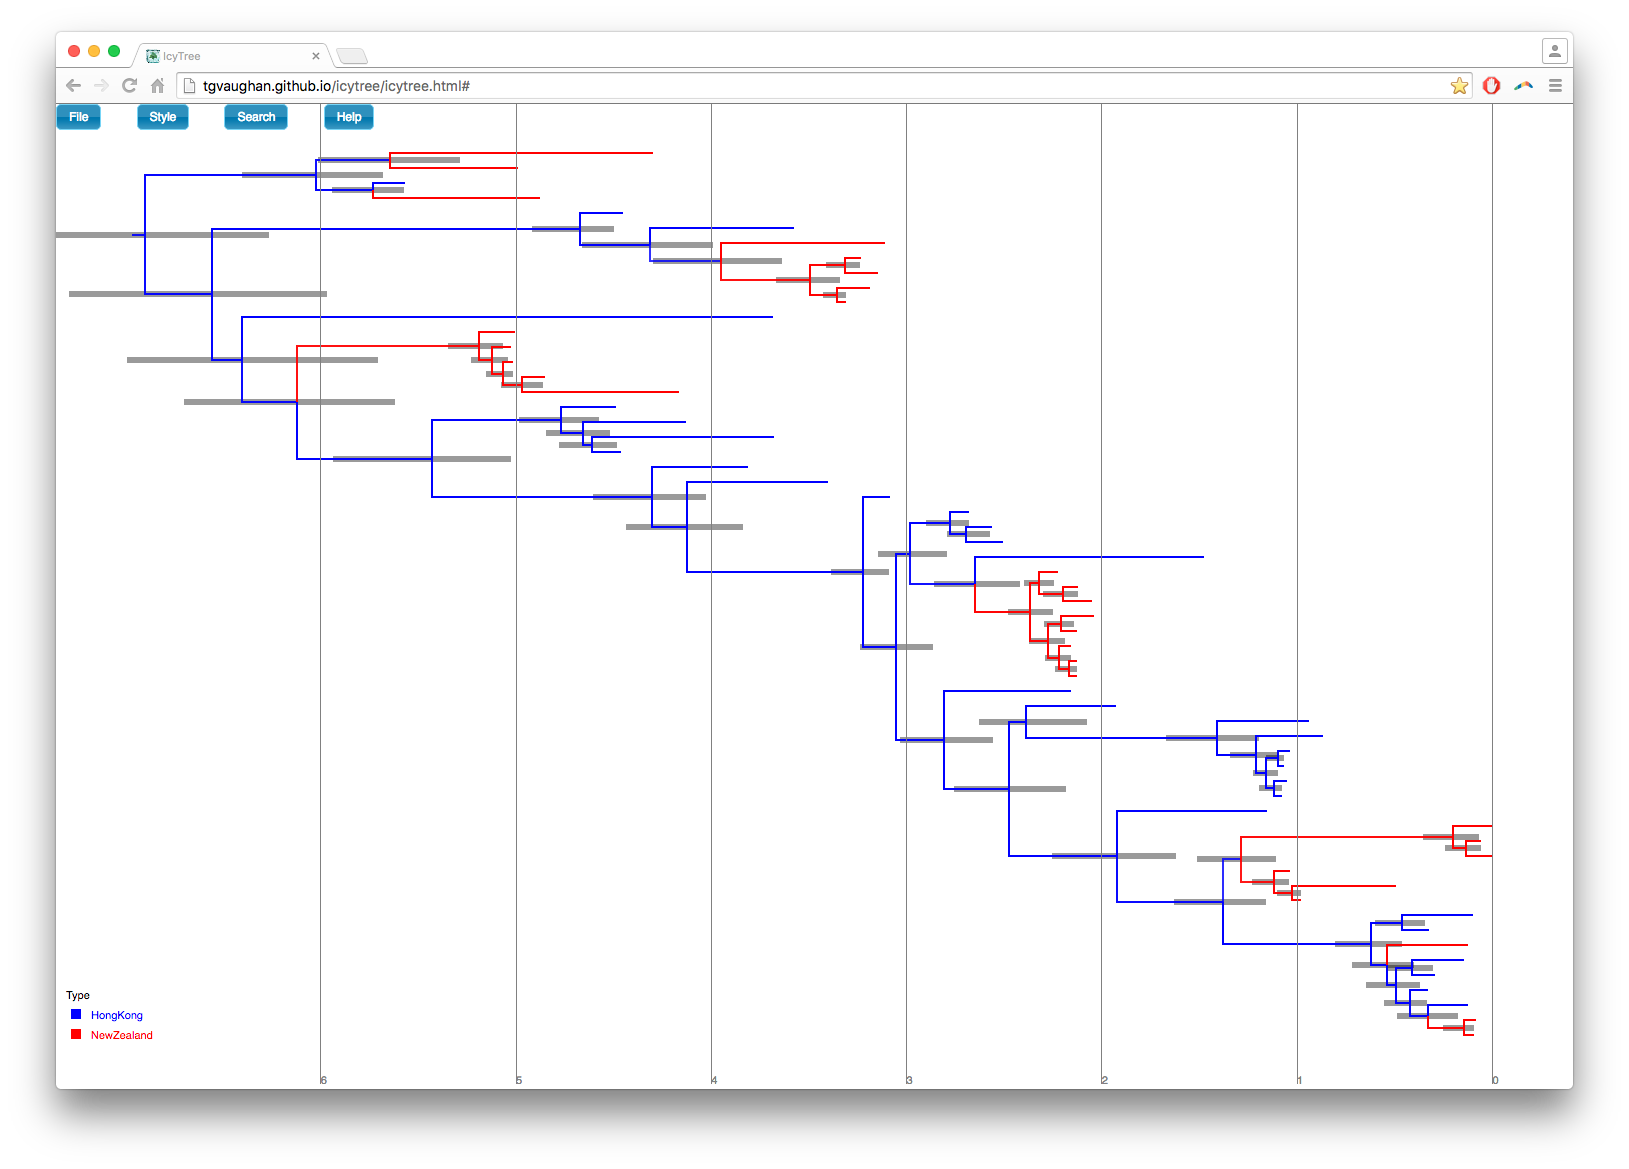
\includegraphics[max width=\textwidth, max height=0.9\textheight]{figures/icyTreeSummary.png}
    \caption{The summary tree in IcyTree.}
    \label{fig:}
\end{figure}

Here we have a full consensus tree annotated by the locations at
coalescence nodes and showing node height uncertainty, with the widths
of the edges representing how certain we can be of the location estimate
at each point on the tree. This is a much more comprehensive summary of
the phylogenetic side of our analysis.

One thing to pay attention to here is that the most probable root
location is given by the summary tree to be Hong Kong (under our model
which assumes that only Hong Kong and New Zealand exist). By hovering
the mouse cursor over the tiny edge above the root will bring up a table
in which posterior probability of the displayed root location
(\lstinline!type.prob!) can be seen to be approximately 90\%. The
analysis therefore strongly supports a Hong Kong origin over a New
Zealand origin.

\href{https://github.com/CompEvol/MultiTypeTree/wiki/Beginner\%27s-Tutorial-\%28short-version\%29\#final-notes}{Very
useful final notes from Tim}

\clearpage

\section{Useful Links}\label{useful-links}

\begin{itemize}

\item
  \href{http://www.beast2.org/book.html}{Bayesian Evolutionary Analysis
  with BEAST 2} \citep{BEAST2book2014}
\item
  \href{https://github.com/denisekuehnert/bdmm}{Multi-type birth-death
  process package} \citep{Kuhnert2016}
\item
  BEAST 2 website and documentation: \url{http://www.beast2.org/}
\end{itemize}

\clearpage



%%%%%%%%%%%%%%%%%%%%%%%
% Tutorial disclaimer %
%%%%%%%%%%%%%%%%%%%%%%%
% Please do not change the license
% Add the author names and relevant links
% Add any other aknowledgments here
\href{http://creativecommons.org/licenses/by/4.0/}{
\includegraphics[scale=0.8]{figures/ccby.pdf}} This tutorial was written by Denise Kühnert for \href{https://taming-the-beast.github.io}{Taming the BEAST} and is licensed under a \href{http://creativecommons.org/licenses/by/4.0/}{Creative Commons Attribution 4.0 International License}. 


%%%%%%%%%%%%%%%%%%%%
% Do NOT edit this %
%%%%%%%%%%%%%%%%%%%%
Version dated: \today



\newpage

%%%%%%%%%%%%%%%%
%  REFERENCES  %
%%%%%%%%%%%%%%%%

\printbibliography[heading=relevref]


\end{document}